% Schutz Solutions Manual

\documentclass{report}
\usepackage[paperwidth=18cm, paperheight=23.6 cm, top = 20mm, bottom = 18mm, left=10mm, right = 10mm]{geometry}
\usepackage{fancyhdr}
\pagestyle{fancy}

\renewcommand{\chaptermark}[1]{%
\markboth{\chaptername
\ \thechapter.\ #1}{}}

\usepackage{graphicx}
\usepackage{amsmath, amsfonts, amssymb, amsthm}
\usepackage{physics}
\usepackage{cancel}
\usepackage{hyphenat}
\usepackage{hyperref}
\usepackage{pgfplots}
\hypersetup{colorlinks, linkcolor = [RGB]{66, 128, 128}, urlcolor = red, linktocpage = true}
\usepackage{enumitem}
\usepackage{tikz}
\usepackage{tkz-euclide}

\usetikzlibrary{calc,arrows,decorations.markings}
\usetkzobj{all}

% \usepackage{charter}

\DeclareMathOperator{\arctanh}{arctanh}

\newlist{subquests}{enumerate}{3}
\setlist[subquests, 1]{leftmargin=*, label = \textbf{\arabic*.}}
\setlist[subquests, 2]{leftmargin=*, label = (\alph*)}
\setlist[subquests, 3]{leftmargin=*, label = (\roman*)}

\renewcommand{\familydefault}{\sfdefault}

\begin{document}

\title{Solutions to \\A First Course in General Relativity (2nd Edition)\\ by Bernard F. Schutz}

\author{Arjit Seth}
\date{}

\maketitle

\chapter{Special relativity}

\begin{subquests}
	\item \emph{Practice with natural units.}
	\begin{subquests}
		\item

		\item

		\item

		\item

		\item

		\item

		\item

		\item		
	\end{subquests}

	\item \emph{More practice with natural units.}
	\begin{subquests}
		\item

		\item

		\item

		\item

		\item
	\end{subquests}

	\item \emph{Spacetime diagrams.}
	\begin{subquests}
		\item

		\item

		\item

		\item

		\item

		\item

		\item

		\item

		\item

		\item

		\item

		\item
	\end{subquests}

	\item \emph{Practice with summation convention}.
	\begin{subquests}
		\item Greek summation.
		\begin{gather*}
			\sum_{\alpha=0}^{3} V_{\alpha}\Delta{x^\alpha} = V_{0}\Delta{t} + V_{1}\Delta{x} + V_{2}\Delta{y} + V_{3}\Delta{z}
		\end{gather*}

		\item Latin summation.
		\begin{gather*}
			\sum_{i=1}^{3} (\Delta{x^i})^2 = (\Delta{x})^2 + (\Delta{y})^2 + (\Delta{z})^2
		\end{gather*}
	\end{subquests}

	\item \emph{More spacetime diagrams.}
	\begin{subquests}
		\item

		\item

		\item

		\item
	\end{subquests}

	\item \emph{Switching indices.}

	\item \emph{Transformations in summation convention.}

	\item \emph{More transformations in summation convention.}
	\begin{subquests}
		\item

		\item

		\item
	\end{subquests}

	\item \emph{Rod in a spacetime diagram.}

	\item \emph{Classifications of spacetime intervals.}
	For this question, we must evaluate the interval between the two space-time points using:
	\begin{subquests}
		\item
		\begin{gather*}
			(\Delta{s})^2 = -(\Delta{t})^2 + (\Delta{x})^2 + (\Delta{y})^2 + (\Delta{z})^2
		\end{gather*}
		
		The separation is null.
		\begin{gather*}
			(\Delta{s})^2 = -(-1-0)^2 + (1-0)^2 + (0-0)^2 + (0-0)
			^2 = 0
		\end{gather*}
		
		\item
		The separation is spacelike.
		\begin{gather*}
			(\Delta{s})^2 = -(-1+1)^2 + (1-1)^2 + (0+1)^2 + (2-0)^2 = 5
		\end{gather*}
		
		\item
		The separation is timelike.
		\begin{gather*}
			(\Delta{s})^2 = -(5-6)^2 + (0-0)^2 + (1-1)^2 + (0-0)^2 = -1
		\end{gather*}
		
		\item
		The separation is null.
		\begin{gather*}
			(\Delta{s})^2 = -(4+1)^2 + (1-1)^2 + (-1+1)^2 + (6-1)^2 = 0
		\end{gather*}
	\end{subquests}

	\item \emph{Hyperbolae in special relativity.}

	\item \emph{Time dilation.}
	\begin{subquests}
		\item

		\item

		\item
	\end{subquests}

	\item \emph{Half-life of pions.}
	The observer is moving with velocity ${\vec v} = -0.999$ with respect to the frame of the pion. The proper time of the half-life of the pion is $2.5 \times 10^{-8}$ seconds. Therefore, the observer will measure a time-dilated value, which is:
	\begin{gather*}
		t = \frac{\tau}{\sqrt{1-v^2}} = \frac{2.5 \times 10^{-8}}{\sqrt{1-(-0.999)^2}}\approx 5.6 \times 10^{-7}\; \mathrm{secs}
	\end{gather*}

	\item \emph{Low-velocity approximations of relativistic effects.}
	\begin{subquests}
		\item Time dilation.
		The time dilation formula is given by:
		\begin{gather*}
			\Delta{t} = \gamma \Delta{\bar{t}} = \frac{\Delta{\bar{t}}}{\sqrt{1-v^2}}
		\end{gather*}
		Expanding the Lorentz factor using a binomial expansion:
		\begin{gather*}
			\frac{1}{\sqrt{1-v^2}} = 1+\frac{v^2}{2}+\frac{3v^4}{8}+\frac{5v^6}{16}+\frac{35v^8}{128}+O(v^9)
		\end{gather*}
		Since $ |{\vec v}| \ll 1$, terms higher than second-order can be discarded, giving:
		\begin{gather*}
			\Delta{t} = \frac{\Delta{\bar{t}}}{\sqrt{1-v^2}}\approx \left(1+\frac{v^2}{2}\right)\Delta{\bar{t}}
		\end{gather*}
		
		\item Length contraction.
		The length contraction formula is given by:
		\begin{gather*}
			\Delta{x} = \frac{\Delta{\bar{x}}}{\gamma} = \Delta{\bar{x}}{\sqrt{1-v^2}}
		\end{gather*}
		Expanding the reciprocal of the Lorentz factor using a binomial expansion:
		\begin{gather*}
			\sqrt{1-v^2} = 1-\frac{v^2}{2}-\frac{v^4}{8}-\frac{v^6}{16}-\frac{5v^8}{128}+O(v^9)
		\end{gather*}
		Since $|{\vec v}| \ll 1$, terms higher than second-order can be discarded, giving:
		\begin{gather*}
			\Delta{x} = \Delta{\bar{x}}{\sqrt{1-v^2}} \approx \left(1-\frac{v^2}{2}\right)\Delta{\bar{x}}
		\end{gather*}
		
		\item Velocity addition.
		The velocity addition formula is given by:
		\begin{gather*}
			w' = \frac{w+v}{1+wv}
		\end{gather*}
		Expanding the denominator using a binomial expansion:
		\begin{gather*}
			\frac{1}{1+wv} = 1-wv+(wv)^2-(wv)^3+(wv)^4-(wv)^5+\order{x^6}
		\end{gather*}
		This gives:
		\begin{gather*}
			w' = [w+v][1-wv+(wv)^2-(wv)^3+(wv)^4-(wv)^5+\order{x^6}]
		\end{gather*}
		Since $|{\vec v}| \ll 1$, terms higher than first-order can be discarded, giving:
		\begin{gather*}
			w' = (w+v)(1-wv) = w + v - wv(w + v)
		\end{gather*}
		This equation would apply for $|{\vec w}| \ll 1$ as well.
		%% Write about error when v = 0.1	
	\end{subquests}

	\item \emph{High-velocity approximations of relativistic effects.}
	\begin{subquests}
		\item Time dilation.
		Inserting the value of $|{\vec v}| = 1-\varepsilon$ into the time dilation and length contraction formulae, we get:
		\begin{gather*}
			\Delta{t} = \frac{\Delta{\bar{t}}}{\sqrt{1-(1-\epsilon)^2}}=\frac{\Delta{\bar{t}}}{\sqrt{2\epsilon-\epsilon^2}} \\
			\Delta{x} = \Delta{\bar{x}}{\sqrt{1-(1-\epsilon)^2}}=\Delta{\bar{x}}{\sqrt{2\epsilon-\epsilon^2}}
		\end{gather*}
		Since $\epsilon$ is very small, its square term can be neglected, giving:
		\begin{gather*}
			\Delta{t} = \frac{\Delta{\bar{t}}}{\sqrt{2\epsilon}} \\
			\Delta{x} = \Delta{\bar{x}}\sqrt{2\epsilon}
		\end{gather*}	
		% Disclaimer
		Note: Schutz's textbook has the incorrect expression presented for length contraction in this question.
% 		%% Write Velocity Addition Expansion
	\end{subquests}

	\item \emph{Deriving relativistic effects from the Lorentz transformations.}

	\item \emph{Pole in a barn problem.}
	\begin{subquests}
		\item

		\item

		\item

		\item

		\item

		\item
	\end{subquests}

	\item \emph{Velocity parametrisation.}
	\begin{subquests}
		\item
		The velocity addition formula is given by:
		\begin{gather*}
			w' = \frac{w+v}{1+wv}
		\end{gather*}
		Substituting the parametrisations $v = \tanh u$ and $w = \tanh U$, we get:
		\begin{gather*}
			w' = \frac{\tanh u + \tanh U}{1+(\tanh u)(\tanh U)} = \tanh(u+U)
		\end{gather*}
		Using the hyperbolic trigonometric identity:
		\begin{gather*}
			\tanh(u+U) = \frac{\tanh u + \tanh U}{1+(\tanh u)(\tanh U)}
		\end{gather*}	
		So the velocity parameters add linearly.

		\item
		% Solving N particle velocity addition problem (NEEDS LOGICAL FIXING)
		Since the speed of the second star with respect to the first star is $v_{2,1} = 0.9 \hspace{3 pt}(c = 1)$, the velocity parameter is $u_{1} = \arctanh(0.9)$. Now, the speed of the third star with respect to the second star is $v_{3,2} = 0.9$, assuming they're all moving away from the first star in the same direction. This makes the velocity parameter $u_{2} = \arctanh(0.9)$. Inductively, the velocity parameter of the $N^{th}$ star with respect to the $(N-1)^{th}$ star will be: $v_{N,N-1} = 0.9 \implies u_{N-1} = \arctan(0.9)$ \\ 
		The velocity of the third star with respect to the reference frame of the first star is:
		\begin{gather*}
		 	v_{3,1} = \tanh(u_{1}+u_{2}) = \tanh(\arctanh(0.9)+\arctanh(0.9)) = \tanh(2\arctanh(0.9))
		\end{gather*}
		Since velocity parameters add linearly, we can show that:
		\begin{gather*}
			\sum_{i=1}^{N-1}u_{i} = \arctanh(v_{N,1})
		\end{gather*}
		Performing induction for {\em N} stars, the speed of the {\em Nth} star with respect to the first star is:
		\begin{gather*}
		 	v_{N,1} = \tanh\left(\sum_{i=1}^{N-1}u_{i}\right)= \tanh[(N-1)\times\arctanh(0.9)]
		\end{gather*}
	\end{subquests}

	\item \emph{Lorentz transformations using the velocity parametrisation.}
	\begin{subquests}
		\item
		A simple substitution into the Lorentz transformation equations in one dimension will yield:
		\begin{gather*}
			\bar{t} = \frac{t-vx}{\sqrt{1-v^2}} = \frac{t-(\tanh u)x}{\sqrt{1-(\tanh u)^2}} = \frac{t-x\tanh u}{\sech u} = t\cosh⁡ u - x\sinh ⁡u \\
			\bar{x} = \frac{x-vt}{\sqrt{1-v^2}} = \frac{x-(\tanh u)t}{\sqrt{1-(\tanh u)^2}} = \frac{x-t\tanh u}{\sech u} = -x\cosh⁡ u + t\sinh ⁡u \\
			\bar{y} = y \\
			\bar{z} = z 
		\end{gather*}
		This looks remarkably similar to the transformation pertaining to rotation of axes in a plane:
		\begin{gather*}
			\mqty[
				\bar{x} \\
				\bar{y} \\
			]
			=
			\mqty[
				\cos\theta & -\sin\theta \\
				\sin\theta & \cos\theta \\	
			]
			\mqty[
				x \\
				y \\
			]
		\end{gather*}
		Writing the parametrised equation in matrix form:
		\begin{gather*}
			\mqty[
				\bar{t} \\
				\bar{x} \\
				\bar{y} \\
				\bar{z} \\
			]
			=
			\mqty[
				\cosh u & -\sinh u & 0 & 0 \\
				\sinh u & \cosh u & 0 & 0 \\
				0 & 0 & 1 & 0 \\
				0 & 0 & 0 & 1 \\
			]
			\mqty[
				t \\
				x \\
				y \\
				z \\
			]
		\end{gather*}
		This implies that a Lorentz transformation can be interpreted as a `hyperbolic rotation' of the space-time axes.


		\item 
		The invariance of the interval is described by the equation:
		\begin{gather*}
			-\bar{t}^{2}+\bar{x}^2=-t^2+x^2
		\end{gather*}
		Substituting the previous result:
		\begin{gather*}
			RHS = (-t^2+x^2)(\cosh^2 u - \sinh^2 u)
		\end{gather*}
		From the identity:  
		\begin{gather*}
			\cosh^2 u - \sinh^2⁡ u = 1
		\end{gather*}
		Therefore
		\begin{gather*}
			RHS=-t^2+x^2
		\end{gather*}
		Hence the interval is invariant under the velocity parametrisation.

		\item
		The analog of the interval is the Euclidean distance:
		\begin{gather*}
		-\bar{t}^2+\bar{x}^2=-t^2+x^2 \Leftrightarrow \bar{x}^2+\bar{y}^2 = x^2 + y^2
		\end{gather*}
		The analog of the invariant hyperbolae, represented by $-t^2+x^2 = a^2$, is a circle of radius $a$, represented by the equation $x^2+y^2 = a^2$.
		So we're dealing with non-Euclidean geometry, which requires adjustment of rules such as the triangle inequality and the Pythagorean Theorem from the Euclidean sense.
	\end{subquests}

	\item \emph{Lorentz transformation matrices.}
	\begin{gather*}
		\mqty[
	 		\bar{t} \\
			\bar{x} \\
			\bar{y} \\
			\bar{z}
		]
		=
		\mqty[
		 		\gamma & -\gamma v & 0 & 0 \\
			 	-\gamma v & \gamma & 0 & 0 \\
				0 & 0 & 1 & 0 \\
			 	0 & 0 & 0 & 1
		]
	 	\mqty[
	 		 t \\
	 		 x \\
	 		 y \\
	 		 z
	 	]
	 		,\;\; \gamma = \frac{1}{\sqrt{1-v^2}}
	\end{gather*}
\end{subquests}

\chapter{Vector analysis in special relativity}

\begin{subquests}
	\item \emph{Practice with index notation.}
	\begin{subquests}
		\item
		\begin{gather*}
			A^{\alpha}B_{\alpha} = A^{0}B_{0} + A^{1}B_{1} + A^{2}B_{2} + A^{3}B_{3} = -4 
		\end{gather*}
		
		\item
		\begin{gather*}
			A^{\alpha}C_{\alpha 0} = 5 - 4 + 6 = 7, \\
			A^{\alpha}C_{\alpha 1} = 
	 		A^{\alpha}C_{\alpha 2} = 
	 		A^{\alpha}C_{\alpha 3}  
		\end{gather*}

		\item 

		\item

		\item

		\item

		\item
	\end{subquests}

	\item \emph{Playing with indices.}
	\begin{subquests}
		\item $\alpha$ is a dummy index. $A^{\alpha}B_{\alpha} = 5$ represents one equation. Change $\alpha$ to $\beta$.

		\item $\bar{\mu}$ is free and $\nu$ is dummy. $A^{\bar \mu} = \Lambda^{\bar \mu}_{\;\nu} A^{\nu}$ represents four equations.

		\item

		\item

	\end{subquests}

	\item \emph{Spatial indices vs. spacetime indices.} Trivial.

	\item \emph{Practice with vectors.}

	\item \emph{Linear independence of vectors.}
	\begin{subquests}
		\item 
		The determinant of the matrix formed form the basis vectors as columns is 1.

		\item No, the fourth component is expressible as a linear combination of the other three.
	\end{subquests}

	\item \emph{Vectors in spacetime diagrams.}

	\item \emph{Basis vectors in index notation.}
	\begin{subquests}
		\item Trivial.

		\item Trivial.
	\end{subquests}

	\item \emph{Frame dependence of two vectors.}
	\begin{subquests}
		\item Applying a Lorentz transformation proves the result trivially.

		\item Subtract the two vectors with the same components in the first frame, the result is the zero vector. Since the Lorentz transformations are linear, the previous result follows.
	\end{subquests}

	\item \emph{Double summation in index notation.} Trivial and painful to type.

	\item \emph{Transformation of basis vectors.}
	Using:
	\begin{gather*}
		A^{\alpha}\pqty{\Lambda^{\bar \beta}_{\;\alpha}\vec{e}_{\bar \beta} - \vec{e}_{\alpha}} = 0
	\end{gather*}
	Let ${\vec A} = (1, 1, 1 , 1)^T$.

	\item \emph{Lorentz transformations using index notation.}
	\begin{subquests}
		\item
		The Lorentz transformation matrix is represented by the symbol:
		\begin{gather*}
			\Lambda^{\bar{\alpha}}_{\;\;\beta} = 
			\mqty[
				\gamma & -\gamma v & 0 & 0 \\
				-\gamma v & \gamma & 0 & 0 \\
				0 & 0 & 1 & 0 \\
				0 & 0 & 0 & 1
			]
		\end{gather*}

		The matrix of $\Lambda^{\nu}_{\;\;\bar{\mu}}$ can be obtained by inverting the signs of $v$ in $\Lambda^{\bar{\alpha}}_{\;\;\beta}$ or by finding the inverse of the Lorentz transformation matrix (using Gaussian elimination). Either way, the resultant matrix is:
		\begin{gather*}
			\Lambda^{\nu}_{\;\;\bar{\mu}} = 
			\mqty[
				\gamma & \gamma v & 0 & 0 \\
				\gamma v & \gamma & 0 & 0 \\
				0 & 0 & 1 & 0 \\
				0 & 0 & 0 & 1
			]
		\end{gather*}
		
		\item
		The components of a four-vector (or any vector, for that matter) transform according to the following law:
		\begin{gather*}
			A^{\bar{\alpha}}=\Lambda^{\bar{\alpha}}_{\;\;\beta}A^{\beta} 
		\end{gather*}
		Evaluating the components:
			\begin{gather*}
				A^{\bar{0}}=
				\Lambda^{\bar{0}}_{\;\;0}A^{0} + \Lambda^{\bar{0}}_{\;\;1}A^{1} +
				\Lambda^{\bar{0}}_{\;\;2}A^{2} + \Lambda^{\bar{0}}_{\;\;3}A^{3}
				= \gamma(A^0-vA^1)\\
				A^{\bar{1}}=
				\Lambda^{\bar{1}}_{\;\;1}A^{1} + \Lambda^{\bar{1}}_{\;\;1}A^{1} +
				\Lambda^{\bar{1}}_{\;\;2}A^{2} + \Lambda^{\bar{1}}_{\;\;3}A^{3}
				= \gamma(A^1-vA^0) \\
				A^{\bar{2}} = A^2  \\
				A^{\bar{3}}	= A^3
			\end{gather*}
		Therefore, ${\vec A} \stackrel{\bar{O}}{\longrightarrow}\left(A^{\bar{0}},A^{\bar{1}},A^{\bar{2}},A^{\bar{3}}\right) = (\gamma(A^0-vA^1),\gamma(A^1-vA^0),A^2,A^3)$\\
		Thus we have applied a Lorentz transformation on a general four-vector.

		\item
		Computation of the expression $\Lambda^{\nu}_{\;\;\bar{\beta}}(-{\vec v})\Lambda^{\bar{\beta}}_{\;\;\alpha}({\vec v}) = \delta^{\nu}_{\;\;\alpha}$ will prove that the matrices are indeed inverses of each other.
			\begin{gather*}
				\Lambda^{0}_{\;\;\bar{0}}\Lambda^{\bar{0}}_{\;\;0} + \Lambda^{0}_{\;\;\bar{1}}\Lambda^{\bar{1}}_{\;\;0} + \Lambda^{0}_{\;\;\bar{2}}\Lambda^{\bar{2}}_{\;\;0} + \Lambda^{0}_{\;\;\bar{3}}\Lambda^{\bar{3}}_{\;\;0} = \delta^{0}_{\;\;0} \\
				\gamma^2- \gamma^2v^2 = \gamma^2(1-v^2) = \frac{1}{1-v^2}(1-v^2) = 1 \\				
				\Lambda^{1}_{\;\;\bar{0}}\Lambda^{\bar{0}}_{\;\;0} + \Lambda^{1}_{\;\;\bar{1}}\Lambda^{\bar{1}}_{\;\;0} + \Lambda^{1}_{\;\;\bar{2}}\Lambda^{\bar{2}}_{\;\;0} + \Lambda^{1}_{\;\;\bar{3}}\Lambda^{\bar{3}}_{\;\;0} = \delta^{1}_{\;\;0} \\
				-v\gamma^2 + v\gamma^2 = 0
			\end{gather*}
		Further computations can be obtained from symmetry or are trivial, and the result follows.

		\item
		The inverse transformation matrix is given by:
		\begin{gather*}
			\Lambda^{\nu}_{\;\;\bar{\mu}} = 
			\mqty[
				\gamma & \gamma v & 0 & 0 \\
				\gamma v & \gamma & 0 & 0 \\
				0 & 0 & 1 & 0 \\
				0 & 0 & 0 & 1
			]
		\end{gather*}
		This is the same result as part (a) because the inverse is merely changing the signs of the velocity in the matrix. Physically, the observer is seeing the object move in the opposite direction. 

		\item
		The following transformation allows us to find $A^{\beta}$ from $A^{\bar{\alpha}}$:
		\begin{gather*}
			A^{\beta} = \Lambda^{\beta}_{\;\;\bar{\alpha}}A^{\bar{\alpha}}
		\end{gather*}
		The components can be easily found using the inverse matrix, and thus the vector \\${\vec A} \stackrel{O}{\longrightarrow}\left(A^{{0}},A^{{1}},A^{{2}},A^{{3}}\right) = (\gamma(A^{\bar{0}}+vA^{\bar{1}}),\gamma(A^{\bar{1}}+vA^{\bar{0}}),A^{\bar{2}},A^{\bar{3}})$\\
		This agrees with the results of the inverse Lorentz transformation.

		\item
		% Change of Indices Identity %% DO IT LATER
		
		\item
		Since vectors can be represented as linear combinations of other vectors, ${\vec e}_{\alpha}$ can be written as (in a different reference frame moving in the opposite direction for investigative purposes in this example):
		\begin{gather*}
			{\vec e}_{\alpha} = \Lambda^{\bar{\beta}}_{\;\;\alpha}{\vec e}_{{\bar{\beta}}}
		\end{gather*}
		Following the same logic, ${\vec e}_{\bar{\beta}}$ can also be written as a linear combination of basis vectors:
		\begin{gather*}
			{\vec e}_{\bar{\beta}} = \Lambda^{\nu}_{\;\;\bar{\beta}}{\vec e}_{\nu}
		\end{gather*}
		Therefore, ${\vec e}_{\alpha}$ can be written as a linear combination of ${\vec e}_{\nu}$:
		\begin{gather*}
			{\vec e}_{\alpha} = \Lambda^{\bar{\beta}}_{\;\;\alpha}\Lambda^{\nu}_{\;\;\bar{\beta}}{\vec e}_{\nu}
		\end{gather*}
		Evaluating the dummy sum over $\bar{\beta}$ results in the following expression:
		\begin{gather*}
			{\vec e}_{\alpha} = \Lambda^{\nu}_{\;\;\alpha}{\vec e}_{\nu}
		\end{gather*}
		Considering that these basis vectors are in the same reference frame, they must be linearly independent by definition. The above expression expresses one basis vector of a reference frame as a linear combination of the other basis vectors in the same reference frame. The only way this is possible if the right-hand expression is the basis vector itself, so the components $\Lambda^{\nu}_{\;\;\alpha}$ must be the Kronecker delta: 
		\begin{gather*}
			{\vec e}_{\alpha} = \delta^{\nu}_{\;\;\alpha}{\vec e}_{\nu}
		\end{gather*}
	\end{subquests}

	\item \emph{Lorentz transformation of vectors.}
	\begin{subquests}
		\item
		The vector ${\vec A} \stackrel{O}{\longrightarrow}(0,-2,3,5).$ The following equation describes the Lorentz transformation of the components of the second frame with respect to the components of the first frame:
		\begin{gather*}
			A^{\bar{\alpha}}=\Lambda^{\bar{\alpha}}_{\;\;\beta}A^{\beta} 
		\end{gather*}
		Using ${\vec A} \stackrel{\bar{O}}{\longrightarrow}\left(A^{\bar{0}},A^{\bar{1}},A^{\bar{2}},A^{\bar{3}}\right) = (\gamma_{1}(A^0-vA^1),\gamma_{1}(A^1-vA^0),A^2,A^3)$, we get:
		\begin{gather*}
			{\vec A} \stackrel{\bar{O}}{\longrightarrow}(\gamma_{1}(0-0.8\times-2),\gamma_{1}(-2-0.8\times0),3,5)
		\end{gather*}
		The Lorentz factor is:
		\begin{gather*}
			\gamma_{1} = \frac{1}{\sqrt{1-0.8^2}} = 1.667 
		\end{gather*}
		Therefore,
		\begin{gather*}
			{\vec A} \stackrel{\bar{O}}{\longrightarrow} (2.667,-3.333,3,5)
		\end{gather*}
				
		\item % Components in second frame
		The components of the vector in frame 3 are:
		\begin{gather*}
				A^{\bar{\bar{\mu}}}=\Lambda^{\bar{\bar{\mu}}}_{\;\;\bar{\alpha}}A^{\bar{\alpha}} 
		\end{gather*}
		Using the previous expression for the components of $A^{\bar{\alpha}}$,
		\begin{gather*}			A^{\bar{\bar{\mu}}}=\Lambda^{\bar{\bar{\mu}}}_{\;\;\bar{\alpha}}\Lambda^{\bar{\alpha}}_{\;\;\beta}A^{\beta}=\Lambda^{\bar{\bar{\mu}}}_{\;\;\beta}A^{\beta}
		\end{gather*}
		We can represent this transformation as a matrix multiplication:
		\begin{gather*}
			\mqty[
		 		A^{\bar{\bar{0}}} \\
				A^{\bar{\bar{1}}} \\
				A^{\bar{\bar{2}}} \\
				A^{\bar{\bar{3}}}
			]
			=
			\mqty[
			 	\gamma_{2} & -\gamma_{2} v_{2} & 0 & 0 \\
				-\gamma_{2} v_{2} & \gamma_{2} & 0 & 0 \\
				0 & 0 & 1 & 0 \\
				0 & 0 & 0 & 1
			]
			\mqty[
			 	\gamma_{1} & -\gamma_{1} v_{1} & 0 & 0 \\
				-\gamma_{1} v_{1} & \gamma_{1} & 0 & 0 \\
				0 & 0 & 1 & 0 \\
				0 & 0 & 0 & 1
			]
		 	\mqty[
		 		A^{0} \\
				A^{1} \\
				A^{2} \\
				A^{3}
		 	]
		\end{gather*}
		with $v_{1} = 0.8$ and $v_{2} = 0.6$. The second Lorentz factor is:
		\begin{gather*}
			\gamma_{2} = \frac{1}{\sqrt{1-0.6^2}} = 1.25 
		\end{gather*}
		Simplifying the matrix, we can compute the matrix $\Lambda^{\bar{\bar{\mu}}}_{\;\;\beta}$ that outlines the stacked Lorentz transformations from frame 1 to frame 3 directly:
		\begin{gather*}
			\mqty[
		 		A^{\bar{\bar{0}}} \\
				A^{\bar{\bar{1}}} \\
				A^{\bar{\bar{2}}} \\
				A^{\bar{\bar{3}}}
			]
			=
			\mqty[
			 	\gamma_{2}\gamma_{1}(1+v_{1}v_{2}) & -\gamma_{2}\gamma_{1}(v_{1}+v_{2}) & 0 & 0 \\
				-\gamma_{2}\gamma_{1}(v_{1}+v_{2}) & \gamma_{2}\gamma_{1}(1+v_{1}v_{2}) & 0 & 0 \\
				0 & 0 & 1 & 0 \\
				0 & 0 & 0 & 1
			]
		 	\mqty[
		 		A^{0} \\
				A^{1} \\
				A^{2} \\
				A^{3}
		 	]
		\end{gather*}
		Solving the system of equations, ${\vec A} \stackrel{\bar{\bar{O}}}{\longrightarrow} (5.835,-6.168,3,5)$.

		\item		
		The magnitude of ${\vec A}$ from its components in $O$ is:
		\begin{gather*}
			|{\vec A}| = -(A^{0})^2 + (A^{1})^2 +(A^{2})^2 +(A^{3})^2 = 38
		\end{gather*}

		\item
		The magnitude of ${\vec A}$ from its components in $\bar{O}$ is:
		\begin{gather*}
			|{\vec A}| = -(A^{\bar{0}})^2 + (A^{\bar{1}})^2 +(A^{\bar{2}})^2 +(A^{\bar{3}})^2 = 38
		\end{gather*}
		Hence the magnitude of the vector, which can be interpreted as the interval between two space-time points, is invariant under a coordinate transformation. Note that the interval is spacelike.
	\end{subquests}

	\item \emph{Composition of Lorentz transformations.}
	\begin{subquests}
		\item
		The Lorentz transformation from $O$ to $\bar{O}$ is given by:
		\begin{gather*}
			A^{\bar{\gamma}}=\Lambda^{\bar{\gamma}}_{\;\;\mu}({\vb v})A^{\mu} 
		\end{gather*}
		The Lorentz transformation from $\bar O$ to $\bar{\bar{O}}$ is given by:
		\begin{gather*}
			A^{\bar{\bar{\alpha}}} = \Lambda^{\bar{\bar{\alpha}}}_{\;\;\bar{\gamma}}({\vb v'})A^{\bar{\gamma}} 
		\end{gather*}
		Since $A^{\bar{\gamma}}$ can be expanded as the Lorentz transformation with respect to frame $O$,
		\begin{gather*}
			A^{\bar{\bar{\alpha}}} = \Lambda^{\bar{\bar{\alpha}}}_{\;\;\bar{\gamma}}({\vb v'})\Lambda^{\bar{\gamma}}_{\;\;\mu}({\vb v})A^{\mu}
		\end{gather*}

		\item		
		Since the expressions can be represented as matrix multiplication,	
		\begin{gather*}
			\Lambda^{\bar{\bar{\alpha}}}_{\;\;\mu} = 	
			\mqty[
				\gamma_{2} & 0 & -\gamma_{2} v_{2} & 0 \\
				 0 & 1 & 0 & 0 \\
				-\gamma_{2} v_{2} & 0 & \gamma_{2} & 0 \\
				0 & 0 & 0 & 1
			]
			\mqty[
				\gamma_{1} & -\gamma_{1} v_{1} & 0 & 0 \\
				-\gamma_{1} v_{1} & \gamma_{1} & 0 & 0 \\
				0 & 0 & 1 & 0 \\
				0 & 0 & 0 & 1
			]
		\end{gather*}
		Evaluating this matrix:
		\begin{gather*}
			\Lambda^{\bar{\bar{\alpha}}}_{\;\;\mu} = 	
			\mqty[
				\gamma_{2}\gamma_{1} & -\gamma_{2}\gamma_{1}v_{1} & -\gamma_{2}v_{2} & 0 \\
				-\gamma_{1}v_{1} & 1 & 0 & 0 \\
				-\gamma_{2}\gamma_{1} v_{2} & 0 & \gamma_{2}\gamma_{1} & 0 \\
				0 & 0 & 0 & 1
			]
		\end{gather*}

		\item 
		$v_{1}$ corresponds to ${\vb v} = 0.6{\vec e_{x}}, v_{2}$ corresponds to ${\vb v'} = 0.8{\vec e_{y}}$ and $\gamma_{1} = 1.25, \gamma_{2} = 1.667.$
		\begin{gather*}
			\Lambda^{\bar{\bar{\alpha}}}_{\;\;\mu} = 	
			\mqty[
				\gamma_{2}\gamma_{1} & -\gamma_{2}\gamma_{1}v_{1} & -\gamma_{2}v_{2} & 0 \\
				-\gamma_{1}v_{1} & 1 & 0 & 0 \\
				-\gamma_{2}\gamma_{1} v_{2} & 0 & \gamma_{2}\gamma_{1} & 0 \\
				0 & 0 & 0 & 1
			]
			=
			\mqty[
				2.084 & -1.250 & -1.334 & 0 \\
				-0.750 & 1 & 0 & 0 \\
				-1.667 & 0 & 2.084 & 0 \\
				0 & 0 & 0 & 1
			]
		\end{gather*}

		\item %% do d) later
		
		\item		
		Evaluating the expression as a matrix multiplication:
		\begin{gather*}
			\Lambda^{\bar{\bar{\alpha}}}_{\;\;\beta} = \Lambda^{\bar{\bar{\alpha}}}_{\;\;\bar{\gamma}}({\vb v})\Lambda^{\bar{\gamma}}_{\;\;\beta}({\vb v'}) =
			\mqty[
				\gamma_{1} & -\gamma_{1} v_{1} & 0 & 0 \\
				-\gamma_{1} v_{1} & \gamma_{1} & 0 & 0 \\
				0 & 0 & 1 & 0 \\
				0 & 0 & 0 & 1
			]
			\mqty[
				\gamma_{2} & 0 & -\gamma_{2} v_{2} & 0 \\
				 0 & 1 & 0 & 0 \\
				-\gamma_{2} v_{2} & 0 & \gamma_{2} & 0 \\
				0 & 0 & 0 & 1
			] \\
			\Lambda^{\bar{\bar{\alpha}}}_{\;\;\beta} = 	
			\mqty[
				\gamma_{1}\gamma_{2} & -\gamma_{1}v_{1} & -\gamma_{1}\gamma_{2} v_{2} & 0 \\
				-\gamma_{1}\gamma_{2}v_{1} & 1 & 0 & 0 \\
				-\gamma_{2}v_{2} & 0 & \gamma_{1}\gamma_{2} & 0 \\
				0 & 0 & 0 & 1
			]
			=
			\mqty[
				2.084 & -0.750 & -1.667 & 0 \\
				-1.250 & 1 & 0 & 0 \\
				-1.334 & 0 & 2.084 & 0 \\
				0 & 0 & 0 & 1
			]
		\end{gather*}
		So the two expressions are not equal, as expected from the non-commutation of matrix multiplication. An interesting point, notice how $\Lambda^{\bar{\bar{\alpha}}}_{\;\;\beta}$ is the transpose of $\Lambda^{\bar{\bar{\alpha}}}_{\;\;\mu}.$ This physically represents a spatial rotation in another reference frame.
	\end{subquests}

	\item{Lorentz transformation as a matrix.}
	\begin{subquests}
		\item
		The direction of $\bar{O}$ is in the negative z-direction, as can be deduced from the previous exercises on Lorentz transformations. Since $\gamma = 1.25$ and $-\gamma v = 0.75 \Rightarrow v = -0.75/1.25 = -0.6$, the direction remaining consistent with the previous observation.

		\item
		While Gaussian elimination will easily provide the inverse matrix, a little physical reasoning immediately leads to the deduction that the inverse is:
		\begin{gather*}
			\begin{bmatrix}
				1.25 & 0 & 0 & -0.75 \\
				0 & 1 & 0 & 0 \\
				0 & 0 & 1 & 0 \\
				-0.75 & 0 & 0 & 1.25
			\end{bmatrix}
		\end{gather*}
		
		\item		
		A convention is introduced here in which the vector will be represented by its component form $A^{\alpha}$. The components in frame $O$ can be found by the following expression:
		\begin{gather*}
			A^{\alpha}=\Lambda^{\alpha}_{\;\;\bar{\beta}}A^{\bar{\beta}} =
			\begin{bmatrix}
				1.25 & 0 & 0 & -0.75 \\
				0 & 1 & 0 & 0 \\
				0 & 0 & 1 & 0 \\
				-0.75 & 0 & 0 & 1.25
			\end{bmatrix}
			\begin{bmatrix}
		 		A^{\bar{0}} \\
				A^{\bar{1}} \\
				A^{\bar{2}} \\
				A^{\bar{3}}
			\end{bmatrix}
			=
			\begin{bmatrix}
				1.25 & 0 & 0 & -0.75 \\
				0 & 1 & 0 & 0 \\
				0 & 0 & 1 & 0 \\
				-0.75 & 0 & 0 & 1.25
			\end{bmatrix}
			\begin{bmatrix}
		 		1 \\
				2 \\
				0 \\
				0
			\end{bmatrix}	
		\end{gather*}
		Where $\Lambda^{\alpha}_{\;\;\bar{\beta}}$ is the inverse transformation matrix above. Therefore, by performing the matrix multiplication, ${\vec A} \stackrel{O}{\longrightarrow}(A^{0},A^{1},A^{2},A^{3}) = (1.25, 2, 0, -0.75).$ Notice how the time component dilates to a larger value and the length in the z-direction (the direction of motion) contracts to a smaller (negative) value, thus displaying the relativistic effects.
	\end{subquests}

	\item \emph{Four-velocity transformations.}
	\begin{subquests}
		\item
		The velocity of the $O$ frame is in the negative x-direction with respect to the MCRF of the particle. Expressing the velocity of the particle in its rest frame as a four-vector ${\vec V} \stackrel{MCRF}{\longrightarrow}(1,0,0,0)$, we can apply the Lorentz transformation:
		\begin{gather*}
			V^{\alpha}=\Lambda^{\alpha}_{\;\;\bar{\beta}}V^{\bar{\beta}} =
			\mqty[
				\gamma & \gamma v & 0 & 0 \\
				\gamma v & \gamma & 0 & 0 \\
				0 & 0 & 1 & 0 \\
				0 & 0 & 0 & 1
			]
			\mqty[
		 		1 \\
				0 \\
				0 \\
				0
			]
			=
			\mqty[
		 		\gamma \\
				\gamma v \\
				0 \\
				0
			]	
		\end{gather*}
		Therefore, ${\vec V} \stackrel{O}{\longrightarrow}(\gamma,\gamma v,0,0)$.
		
		\item
		Observation suggests that an arbitrary three-velocity ${\vb v} =  v^x {\vb e}_x + v^y {\vb e}_y + v^z {\vb e}_z$ will result in the vector ${\vec v} \stackrel{O}{\longrightarrow}(\gamma,\gamma v^{x},\gamma v^{y},\gamma v^{z})$, where $\gamma = \frac{1}{\sqrt{1-|{\vb v}|^2}}$ after a Lorentz transformation is applied on it from its MCRF. This is justified by the observation that the only non-zero component of the four-velocity vector in the MCRF is the time component.

		\item		
		$ \vb v = \frac{1}{\gamma}(U^{1}, U^{2}, U^{3})$.

		\item		
		The three-velocity can be obtained by dividing the spacial components of the four-velocity with the time component, therefore ${\vb v} = (0.5,0.5,0.5)$.
	\end{subquests}

	\item \emph{Velocity addition formula.}
	\begin{gather*}
		U^{\bar t} = \frac{U^{t} + WU^{x}}{\sqrt{1-W^{2}}} \\
		U^{\bar x} = \frac{U^{x} + WU^{t}}{\sqrt{1-W^{2}}} \\
		\frac{U^{\bar x}}{U^{\bar t}} = \frac{U^{x} + WU^{t}}{U^{t} + WU^{x}} = \frac{v + W}{1 + vW}
	\end{gather*}

	\item \emph{Four-velocity vectors.}
	\begin{subquests}
		\item

		\item
	\end{subquests}

	\item \emph{Properties of different vectors.}
	\begin{subquests}
		\item

		\item
	\end{subquests}
	
	\item \emph{Uniformly accelerated motion.}
	\begin{subquests}
		\item

		\item
		Assuming the body is uniformly accelerated along the x-axis, the velocity and acceleration in the observer's MCRF from $\vec v \cdot \vec a = 0$ are given by:
		\begin{gather*}
			\vec v \stackrel{MCRF}{\longrightarrow}(1, 0, 0, 0) \hspace{20 pt} \vec a \stackrel{MCRF}{\longrightarrow}(0, \alpha, 0, 0)
		\end{gather*}
		Measuring the velocity in the observer $\bar O$'s frame of reference:
		\begin{gather*}
			\vec v \stackrel{\bar O}{\longrightarrow}(\gamma, \gamma v, 0, 0)
		\end{gather*}
		The acceleration in this reference frame is given by:
		\begin{gather*}
			\vec a \stackrel{\bar O}{\longrightarrow}(\gamma v \alpha, \gamma \alpha, 0, 0) 
		\end{gather*}
		To find the acceleration in terms of the velocity derivative, we must differentiate the velocity with respect to the proper time in this frame:
		\begin{gather*}
			\vec a = \dv{\vec v}{\tau} \stackrel{\bar O}{\longrightarrow}
			\dv{\tau}(\gamma, \gamma v, 0, 0) = 
			\dv{v}{\tau}(v\gamma^{3}, v^{2}\gamma^{3} + \gamma, 0, 0) =
			\gamma^2\dv{v}{\tau}(v, 1, 0, 0)
		\end{gather*}
		But $\dd{\tau} = \dd{t}/\gamma$, giving:
		\begin{gather*}
			\vec a \stackrel{\bar O}{\longrightarrow}\gamma^{2}\dv{v}{t}(v\gamma^{2}, v^{2}\gamma^{2} + 1, 0, 0) =
			\gamma^{4}\dv{v}{t}(v, 1, 0, 0)
		\end{gather*}
		Equating the components, we get:
		\begin{gather*}
			\alpha = \gamma^{3}\dv{v}{t}
		\end{gather*}
		Integrating the differential equation:
		\begin{gather*}
			\int^{t}_{0} \alpha \dd{t} = \int^v_0 \frac{1}{(1-v^{2})^{\frac{3}{2}}} \dd{v} 
		\end{gather*}
		This can be solved by making the substitution (without adjusting the limits) $v = \sin \theta \rightarrow \dd{v} = \cos\theta\dd{\theta}$:
		\begin{gather*}
			\alpha t = \int^v_0 \sec^{2}\theta\dd{\theta} = \eval[\tan\theta|^v_0
		\end{gather*}
		The initial velocity is zero. The substitution can be reversed by using the following right triangle: \\
		\begin{center}
			\begin{tikzpicture}[scale=.8]
				\tkzInit[xmax=5,ymax=3] %\tkzClip[space=.5]
				\tkzDefPoint(0,0){A} \tkzDefPoint(4,0){B}
				\tkzDrawTriangle[pythagore](A,B)
				\tkzGetPoint{C}
				\tkzLabelSegment[below,font=\footnotesize](A,B){$\sqrt{1 - v^2}$}
				\tkzLabelSegment[above,font=\footnotesize](A,C){$1$}
				\tkzLabelSegment[right,font=\footnotesize](B,C){$v$}
				\tkzMarkAngle[fill= blue!20,size=1.4cm,opacity=.5](B,A,C)
				\tkzLabelAngle[pos=0.8](B,A,C){$\theta$}
			\end{tikzpicture}
		\end{center}
		This gives the expression:
		\begin{gather*}
			\alpha t = \frac{v}{\sqrt{1-v^2}} \bigg|^v_0 =  \frac{v}{\sqrt{1-v^2}}
		\end{gather*}
		Solving for $v$, which is the speed at time $t$:
		\begin{gather*}
			v = \frac{\alpha t}{\sqrt{1 + \alpha^2 t^2}}
		\end{gather*}
		The distance is given by:
		\begin{gather*}
			\dv{s}{t} = \frac{\alpha t}{\sqrt{1 + \alpha^2 t^2}} \\
			\int^x_0 \;\dd{s} = \int^t_0 \frac{\alpha t}{\sqrt{1 + \alpha^2 t^2}}\dd{t}
		\end{gather*}
		Using the substitution $\alpha t = \tan\theta \longrightarrow \alpha\dd{t} = \sec^2 \theta\dd{\theta}$
		\begin{gather*}
			x = \frac{1}{\alpha}\int^t_0 \sec\theta\tan\theta\dd{\theta} = \sec\theta\big|^t_0 = 
			\frac{\sec\arctan(\alpha t)\big|^t_0}{\alpha}
		\end{gather*}
		The expression can be evaluated using a different right triangle:
		\begin{center}
			\begin{tikzpicture}[scale=.8]
				\tkzInit[xmax=5,ymax=3] %\tkzClip[space=.5]
				\tkzDefPoint(0,0){A} \tkzDefPoint(4,0){B}
				\tkzDrawTriangle[pythagore](A,B)
				\tkzGetPoint{C}
				\tkzLabelSegment[below,font=\footnotesize](A,B){$1$}
				\tkzLabelSegment[above,font=\footnotesize, rotate = 36.86](A,C){$\sqrt{1+\alpha^2 t^2}$}
				\tkzLabelSegment[right,font=\footnotesize](B,C){$\alpha t$}
				\tkzMarkAngle[fill= blue!20,size=1.4cm,opacity=.5](B,A,C)
				\tkzLabelAngle[pos=0.8](B,A,C){$\theta$}
			\end{tikzpicture}
		\end{center}
		\begin{gather*}
			x = \frac{1}{\alpha}\left(\sqrt{1+\alpha^2 t^2} - 1\right)
		\end{gather*}
		The time required to reach $v = 0.999$ is, from equation 2.8i:
		\begin{gather*}
			t = \frac{v}{\alpha \sqrt{1-v^2}} = \frac{0.999}{10\sqrt{1-0.999^2}}\times3\times10^8 = 6.703\times10^8 s 
		\end{gather*}
		
		\item		
		Following the hint, we must perform the integration along the body's world line using the acceleration:
		\begin{gather*}
			\int^{\tau}_0\alpha\dd{\tau} =  \int^v_0 \gamma^2\dd{v} = \int^v_0 \frac{\dd{v}}{1-v^2}
		\end{gather*}
		While this integral is easily solvable via partial fractions, there is a hyperbolic solution we should follow in the spirit of special relativity:
		\begin{gather*}
			\tau = \frac{1}{\alpha}\eval[\arctanh(v)|^v_0 = \frac{\arctanh(v)}{\alpha} = \frac{1}{\alpha}\arctanh \left(\frac{\alpha t}{\sqrt{1 + \alpha^2 t^2}}\right)
		\end{gather*}
		Note that we obtain the well-known rapidity parametrisation with $v = \tanh (\alpha \tau)$. \\
		The proper time elapsed by the time the speed $v = 0.999$ is $$\tau = \frac{\left(3 \times 10^8\right)}{10}\arctanh(0.999) = 1.14 \times 10^8$$ seconds, which is about 3.6 years.
		% Add final answer later
	\end{subquests}

	\item \emph{Motion of a wheel?}
	\begin{gather*}
		\vb{v} = \pqty{a + b\omega \cos \omega t}\vb{e}_{x} + \pqty{-b\omega\sin \omega t}\vb{e}_y
	\end{gather*}

	\item \emph{}
	Calculating the interval described by the parametric equations:
	\begin{gather*}
		\dd{s^{2}} = - \dd{t^{2}} + \dd{x^{2}} = \dd{\lambda^2}\left[-\cosh^2\left(\frac{\lambda}{a}\right) + \sinh^2\left(	\frac{\lambda}{a}\right)\right] = -\dd{\lambda^{2}} = -\dd{\tau^{2}}
	\end{gather*}
	Which indicates that $\lambda$ is indeed the proper time $\tau$. \\
	The four-velocity is given by $\vec U = \dd{\vec x}/\dd{\tau}$.
	\begin{gather*}
		\vec U = \dv{\vec x}{\tau} = \dv{\vec x}{\lambda} \stackrel{O} \longrightarrow
		\left(\cosh\left(\frac{\lambda}{a}\right), \sinh\left(\frac{\lambda}{a}\right), 0, 0 \right) 
	\end{gather*}
	The four-acceleration is given by $\vec a = \dd[2]{\vec x}/\dd{\tau}^2$
	\begin{gather*}
		\vec a = \dv[2]{\vec x}{\tau} = \dv[2]{\vec x}{\lambda} \stackrel{O} \longrightarrow \dv{\lambda}\left(\cosh\left(\frac{\lambda}{a}\right), \sinh\left(\frac{\lambda}{a}\right), 0, 0 \right) \\ = \frac{1}{a} \left(\sinh\left(\frac{\lambda}{a}\right), \cosh\left(\frac{\lambda}{a}\right), 0, 0 \right) = \frac{1}{a^2}\left(t(\lambda), x(\lambda), 0, 0\right)
	\end{gather*}
	This is cyclic motion in Minkowski spacetime.

	\item \emph{Energies and momenta of particles.}
	\begin{subquests}
		\item
		The four-momentum is given by $\vec p \stackrel{O} \longrightarrow (E, p^1, p^2, p^3)$. So the energy is 4 kg. \\
		The rest mass can be found using:
		\begin{gather*}
			E^2 = m^2 + \sum^3_{i=3} (p^i)^2 \longrightarrow m = \sqrt{E^2 - \sum^3_{i=3}(p^i)^2} = \sqrt{4^2 - 1^2 - 1^2} = 3.74 \;\mathrm{kg} 
		\end{gather*}
		The three-velocity $\vb v$ can be found from dividing the momentum components by the energy components using the definition: $\vec p = m\vec U$, giving:
		\begin{gather*}
			{\vb v} = 0.25\vb{e}_x + 0.25\vb{e}_y
		\end{gather*}
		
		\item		
		Following the conservation of four-momentum, we get $\vec p_5 \stackrel{O}\rightarrow (3, -0.5, 1, 0)$. Its energy is 3 kg, its rest mass is approximately 2.78 kg, its three-velocity is: $\vb v = -1/6\vb{e}_x + 1/3\vb{e}_y$.\\\\
		The CM frame is defined as the one in which the momentum components of the four-momentum are zero and the energy component is the total energy of the system. This can be found by summing the components of the particles before or after the collision giving $\vec p_M \rightarrow (5, 0, 1, 0)$.\\\\
		This means that the three-velocity of the CM frame must be $\vb v_2 = 0.2\vb{e}_y$.
	\end{subquests}

	\item \emph{Approximate energy of a particle.}
	The energy is given by:
	\begin{gather*}
		E = \frac{m}{\sqrt{1-|{\vb v}|^2}}
	\end{gather*}
	Where $m$ is the rest mass (which represents the rest energy $E_0 = mc^2$). \\
	Using the series expansion for: $$\frac{1}{\sqrt{1 + x}} = 1-\frac{x}{2} + \frac{3x^2}{8} - \frac{5x^3}{16} + \dots \;,\; |x| < 1 $$
	\begin{gather*}
		E = m\left[1 + \frac{1}{2}|{\vb v}|^2 + \frac{3}{8}|{\vb v}|^4 + \order{\abs{\vb v}^6} \right]
	\end{gather*}
	To find the $|\vb v|$ value for which the fourth order term is equal to half of the Newtonian kinetic energy, we must solve:
	\begin{gather*}
		\frac{1}{4}m|{\vb v}|^2 = \frac{3}{8}m|{\vb v}|^4
	\end{gather*}
	Which gives $|{\vb v}| = \sqrt{2/3} \approx 0.816$.

	\item \emph{Electron-positron annihilation.}
	Take an electron with three-velocity ${\vb v}_1 = 0.5{\vb e}_x + 0.5{\vb e}_y$ and a positron with three-velocity ${\vb v}_2 = 0.5{\vb e}_x - 0.5{\vb e}_y$ in the reference frame $O$. To find the four-momentum of each particle, we must first find their four-velocities:
	\begin{gather*}
		\gamma_1 = \gamma_2 = \frac{1}{\sqrt{1 - |{\vb v}_1|^2}} = \frac{1}{\sqrt{1 - 0.707^2}} \approx 1.414 
	\end{gather*}
	This gives:
	\begin{gather*}
		\vec U_1 \stackrel{O}\longrightarrow (1.414, 0.707, 0.707, \; \vec U_2 = \stackrel{O}\longrightarrow (1.414, 0.707, -0.707, 0)
	\end{gather*}
	The masses of an electron and positron are the same ($m$ here). So the four-momentum of each particle is:
	\begin{gather*}
		\vec p_1 = m \vec U_1, \; \vec p_2 = m \vec U_2
	\end{gather*} 
	The total four-momentum of the system is:
	\begin{gather*}
		\vec p_1 + \vec p_2 \stackrel{O}\longrightarrow m(2.828, 1.414, 0, 0)
	\end{gather*}
	The CM frame is then:
	\begin{gather*}
		{\vb v} = 0.5{\vb e}_x
	\end{gather*}
	The four-momentum in the CM frame is:
	\begin{gather*}
		\vec p_1 + \vec p_2 \stackrel{CM}\longrightarrow (2.828, 0, 0, 0)
	\end{gather*}
	Now, this frame observes a collision of particles in the y-axis and an emission of a photon in the x-axis, which has a momentum. But the conservation of momentum dictates that this is impossible; however, emission of two photons at equal angles along the line of collision will conserve momentum.

	\item \emph{The Doppler effect.}
	\begin{subquests}
		\item
		The four-momentum of the photon in $O$'s frame is:
		\begin{gather*}
			\vec p \stackrel{O}\longrightarrow (p^0, p^1, p^2, p^3) = (E, E\cos\theta, E\sin\theta, 0) =(h\nu, h\nu\cos\theta, h\nu\sin\theta, 0)
		\end{gather*}
		Applying the Lorentz transformation to find the energy component $p^{\bar 0}$ in $\bar O$'s frame:
		\begin{gather*}
			p^{\bar 0} = h{\bar \nu} = \gamma(E - Ev\cos\theta) = \gamma(h\nu - h\nu v\cos\theta)
		\end{gather*}
		\begin{gather*}
			\frac{\bar \nu}{\nu} = \frac{1 - v\cos\theta}{\sqrt{1-v^2}}
		\end{gather*}
		
		\item
		For no Doppler shift, we must have the condition ${\bar \nu}/{\nu} = 1$. Using this condition in the previous derivation:
		\begin{gather*}
			\sqrt{1-v^2} = 1 - v\cos\theta
		\end{gather*}
		This gives the quadratic equation
		\begin{gather*}
			\cos^2\theta -\frac{2}{v}\cos\theta + 1 = 0
		\end{gather*}
		Solving the equation (keeping in mind that $|\cos\theta| < 1 $):
		\begin{gather*}
			\cos\theta = \frac{1 - \sqrt{1-v^2}}{v} \longrightarrow \theta = \arccos \left(\frac{1 - \sqrt{1-v^2}}{v} \right)
		\end{gather*}
		
		\item
		Eq. 2.35: $-\vec p \cdot \vec U_{obs} = -\vec p \cdot \vec e_{\bar 0} = \bar E$, Eq. 2.38: $E = h\nu$. The observer frame's velocity is:
		\begin{gather*}
			\vec U_{obs} \stackrel{O}\longrightarrow (\gamma, -\gamma v, 0, 0)
		\end{gather*}
		So, now we just have to take the dot product:
		\begin{gather*}
			\bar E = h{\bar \nu} = -\vec p \cdot \vec U_{obs} = -\left(-\gamma p^0 + \gamma vp^1\right) = \frac{h\nu - h\nu v \cos\theta}{\sqrt{1-v^2}}
		\end{gather*}
		Which (more neatly) gives the same result:
		\begin{gather*}
			\frac{\bar \nu}{\nu} = \frac{1 - v\cos\theta}{\sqrt{1-v^2}}
		\end{gather*}
	\end{subquests}

	\item \emph{Energy required to accelerate a particle.}

	\item \emph{Acceleration after heat addition.}

	\item \emph{Properties of vectors under Lorentz transformations.}
	\begin{subquests}
		\item
		Applying the Lorentz transformation:
		\begin{gather*}
			\vec A \stackrel{\bar O}\longrightarrow (5.5, -2.5, -1, 0), \;\; 
			\vec B \stackrel{\bar O}\longrightarrow (-4.75, 5.25, 1, 6), \;\; 
			\vec C \stackrel{\bar O}\longrightarrow (4, -4, 0, 0)
		\end{gather*}
		
		\item		
		\begin{gather*}
			\vec A \cdot \vec B \stackrel{\bar O} = -(-4.75 \times 5.5) + (-2.5 \times 5.25) + (-1 \times 1) + (0 \times 6) = 12 \\
			\vec B \cdot \vec C \stackrel{\bar O} = -(-4.75 \times 4) + (-5.25 \times -4) + (1 \times 0) + (6 \times 0) = 40 \\
			\vec A \cdot \vec C \stackrel{\bar O} = -(5.5 \times 4) + (-2.5 \times -4) + (-1 \times 0) + (0 \times 0) = -12 \\
			\vec C \cdot \vec C \stackrel{\bar O} = -(4)^2 + (-4)^2 = 0
		\end{gather*}
		The dot products in the original frame $O$ are as follows:
		\begin{gather*}
			\vec A \cdot \vec B \stackrel{O} = -(5 \times -2) + (1 \times 3) + (-1 \times 1) + (0 \times 6) = 12 \\ 
			\vec B \cdot \vec C \stackrel{O} = -(-2 \times 2) + (3 \times -2) + (1 \times 0) + (6 \times 0) = 40 \\
			\vec A \cdot \vec C \stackrel{O} = -(5 \times 2) + (1 \times -2) + (-1 \times 0) + (0 \times 0) = -12 \\
			\vec C \cdot \vec C \stackrel{O} = -(2)^2 + (-2)^2 = 0 	
		\end{gather*}
		 
		Clearly the dot products are frame-invariant.

		\item		
		$ \vec A^2 \stackrel{O} = -(5)^2 + (1)^2 + (-1)^2 = -23 $, so $\vec A$ is timelike.\\
		$ \vec B^2 \stackrel{O} = -(-2)^2 + (3)^2 + (1)^2 + (6)^2 = 42 $, so $\vec B$ is spacelike.\\
		$ \vec C^2 \stackrel{O} = -(2)^2 + (-2)^2 = 0 $, so $\vec C$ is lightlike.
	\end{subquests}

	\item \emph{Derivative of the calar product of the four-velocity.}
	Using the relevant equations, we expand both sides of:
	$$ \dv{\tau}(\vec U \cdot \vec U) = 2\vec U \cdot \dv{\vec U}{\tau} $$
	\begin{gather*}
		\dv{\tau}\left[-(U^0)^2 + (U^1)^2 + (U^2)^2 + (U^3)^2\right] = -2U^0\dv{U^0}{\tau} + 2U^1\dv{U^1}{\tau} + 2U^2\dv{U^2}{\tau} + 2U^3\dv{U^3}{\tau}
	\end{gather*}
	Differentiating the components on the left side using the chain rule gives the right side.

	\item \emph{Energy and momentum of a rocket ship travelling in an arbitrary direction.}
	\begin{subquests}
		\item
		To solve this problem, we must figure out the general Lorentz transformation for four dimensions. A physical property we must realise about the transformations is that only the parallel component of the spatial vector is contracted and its perpendicular component is left untouched. We can describe the vectorial Lorentz transformations with $\gamma = 1/\sqrt {1-|{\vb v}|^2}$ as follows:
		\begin{gather*}
			\bar t = \gamma (t - {\vb r}_{\parallel}\cdot {\vb v}) \\
			{\vb {\bar r}}_{\parallel} = \gamma ({\vb r}_{\parallel} - {\vb v} t) \\
			{\vb {\bar r}}_{\perp} = {\vb r}_{\perp}
		\end{gather*}
		To find the parallel and perpendicular components, we must use the unit velocity vector $\vb u = v/|v|$ and its projections:
		\begin{gather*}
			{\vb r}_{\parallel} = (\vb r \cdot u)u \\
			{\vb r}_{\perp} = \vb r - (r \cdot u)u
		\end{gather*}
		Substituting these expressions:
		\begin{gather*}
			{\bar t} = \gamma [t - (\vb r \cdot u)u \cdot {\vb v}] \\
			\vb{\bar r}_{\parallel} = \gamma [({\vb r \cdot u)u -} t{\vb v}]  \\
			\vb{\bar r}_{\perp} = \vb r - (r \cdot u)u \\
			\vb{\bar{r}} = \vb{\bar{r}}_{\parallel} +\vb{\bar r}_{\perp} = \pqty{\vb r + (\gamma -1)(\vb r \cdot u)u - \gamma t\vb v}
		\end{gather*}
		Evaluating these expressions in Cartesian components (in the time and x-direction for simplicity; the rest can be figured out via symmetry):
		\begin{gather*}
			{\bar t} = [\gamma]t + [-\gamma v_x] x  + [-\gamma v_y] y + [-\gamma v_z] z \\
			\bar x = [-\gamma v_x] t + \left[1 + (\gamma -1)\frac{v_x^2}{|{\vb v}|^2}\right]x + \left[(\gamma - 1)\frac{v_x v_y}{|{\vb v}|^2}\right]y	+ \left[(\gamma - 1)\frac{v_x v_z}{|{\vb v}|^2}\right]z
		\end{gather*}
		Writing $\alpha = (\gamma -1)/|{\vb v}|^2$ and arranging the other components into $ V^{\bar \beta} = \Lambda^{\bar \beta}_{\;\;\alpha} V^{\alpha}$ as:
		\begin{gather*}
			\mqty[
		 		\bar{t} \\
				\bar{x} \\
				\bar{y} \\
				\bar{z}
			] =
			\mqty[
				\gamma & -\gamma v_x & -\gamma v_y & -\gamma v_z \\
				-\gamma v_x & 1 + \alpha {v}^2_x & \alpha v_x v_y & \alpha v_x v_z \\
				-\gamma v_y & \alpha v_y v_x & 1 + \alpha {v}^2_y & \alpha v_y v_z \\
				-\gamma v_z & \alpha v_z v_x & \alpha v_z v_y & 1 + \alpha {v}^2_z
			]
			\mqty[
		 		{t} \\
				{x} \\
				{y} \\
				{z}
			] 	
		\end{gather*}
		The three-velocity ${\vb v} = 0.5{\vb e}_x + 0.5{\vb e}_y + 0.5{\vb e}_z$ in this question and the Lorentz transformation is $\Lambda^{\bar \beta}_{\;\;\alpha}$ with $\gamma = 2$ and $\alpha = 4/3$. To go to the MCRF, $ {\vec V} \stackrel{MCRF}\longrightarrow (1, 0, 0, 0)$, which follows through when multiplying $ {\vec V} \stackrel{O}\longrightarrow (2, 1, 1, 1) $ by the Lorentz transformation:
		\begin{gather*}
			\mqty[
		 		{1} \\
				{0} \\
				{0} \\
				{0}
			] =
			\mqty[
				2 & -1 & -1 & -1 \\
				-1 & 4/3 & 1/3 & 1/3 \\
				-1 & 1/3 & 4/3 & 1/3 \\
				-1 & 1/3 & 1/3 & 4/3
			]
			\mqty[
		 		{2} \\
				{1} \\
				{1} \\
				{1}
			]
		\end{gather*}
		Using this transformation to transform the cosmic ray's momentum ${\vec P} \stackrel{O} \longrightarrow (300, 299, 0, 0) \times 10^{-27}$ kg to the MCRF of the rocket ship:
		\begin{gather*}
			\mqty[
		 		{301} \\[0.3 pt]
				{296/3} \\[0.3 pt]
				{-601/3} \\[0.3 pt]
				{-601/3}
			] =
			\mqty[
				2 & -1 & -1 & -1 \\
				-1 & 4/3 & 1/3 & 1/3 \\
				-1 & 1/3 & 4/3 & 1/3 \\
				-1 & 1/3 & 1/3 & 4/3
			]
			\mqty[
		 		{300} \\[0.3 pt]
				{299} \\[0.3 pt]
				{0} \\[0.3 pt]
				{0}
			]
		\end{gather*}
		Which gives ${\vec P} \stackrel{MCRF} \longrightarrow (301, 296/3, -601/3, -601/3) \times 10^{-27}$ kg \\\\
		
		\item
		Using $-{\vec P} \cdot \vec V = {\mathrm{\bar E}} = -(-300 \times 2 + 299 \times 1) \times 10^{-27} = 301 \times 10^{-27}$, which is the energy of the cosmic ray.

		\item The second one, since it only involves a computation of a dot product in the MCRF, which is the evaluation of only one component.
	\end{subquests}

	\item \emph{Reflection from a mirror.}
	This is elementary conservation of four-momentum. The initial four-momentum of the photon (for a vertical mirror to the right of the photon) is given by:
	\begin{gather*}
		\vec p_1 \stackrel{O}\longrightarrow (h\nu, h\nu\cos\theta, h\nu\sin\theta, 0)
	\end{gather*}
	After reflection, its final four-momentum is:
	\begin{gather*}
		\vec p_2 \stackrel{O}\longrightarrow (h\nu, -h\nu\cos\theta, h\nu\sin\theta, 0)
	\end{gather*}
	The change in momentum is thus:
	\begin{gather*}
		\vec p_2 - \vec p_1 \stackrel{O}\longrightarrow (0, -2h\nu\cos\theta, 0, 0)
	\end{gather*}
	Therefore, the momentum transferred to the mirror is $2h\nu\cos\theta$ by conservation of four-momentum. If the photon were absorbed, the momentum transferred to the mirror would be $-h\nu \cos\theta \vb{e}_x - h\nu \sin\theta \vb{e}_y$.

	\item \emph{Compton scattering.}
	The four-momentum components of the photon and electron before the collision are:
	\begin{gather*}
		\vec p_1 = (h\nu_i, h\nu_i, 0, 0) \;\;\; \vec p_2 = (m, 0, 0, 0)
	\end{gather*}
	The four-momentum components of the scattered photon and electron after the collision are:
	\begin{gather*}
		\vec p_3 = (h\nu_f, h\nu_f \cos\theta, h\nu_f \sin\theta, 0) \;\;\; \vec p_4 = (p^0, p^1, p^2, p^3)
	\end{gather*}
	Using the conservation of four-momentum, the four-momentum of the scattered electron is:
	\begin{gather*}
		\vec p_4 = \vec p_1 + \vec p_2 - \vec p_3 =
		\begin{bmatrix}
			h(\nu_i - \nu_f) + m \\
			h\nu_i - h\nu_f \cos\theta \\
			-h\nu_f \sin\theta \\
			0
		\end{bmatrix}
	\end{gather*}
	Now, we know that the four-momentum of a particle is $\vec p \cdot \vec p = -m^2$. So, finding the magnitude of the scattered electron's four-momentum:
	\begin{gather*}
		{\vec p}_4 \cdot {\vec p}_4 =
		\begin{bmatrix}
			h(\nu_i - \nu_f) + m \\
			h\nu_i - h\nu_f \cos\theta \\
			-h\nu_f \sin\theta \\
			0
		\end{bmatrix} \cdot
		\begin{bmatrix}
			h(\nu_i - \nu_f) + m \\
			h\nu_i - h\nu_f \cos\theta \\
			-h\nu_f \sin\theta \\
			0
		\end{bmatrix} \\
		= -(h(\nu_i - \nu_f) + m)^2 + (h\nu_i - h\nu_f \cos\theta)^2 + (-h\nu_f \sin\theta)^2 = -m^2
	\end{gather*}
	Expanding the expression and cancelling terms, we're left with:
	\begin{gather*}
		-2h^2\nu_i \nu_f (1-\cos\theta) + 2hm(\nu_i - \nu_f) = 0
	\end{gather*}
	Rearranging the terms, we get the final expression for the frequency shift in Compton scattering:
	\begin{gather*}
		\frac{1}{\nu_f} = \frac{1}{\nu_i} + \frac{h}{m}(1-\cos\theta)
	\end{gather*}

	\item \emph{Cosmic radiation.}

	\item \emph{Properties of the scalar product.} The scalar product is bilinear, and satisfies these properties by definition.

	\item \emph{Transformation of the metric tensor.} Trivial.
\end{subquests}

\chapter{Tensor analysis in special relativity}

\begin{subquests}
	\item \emph{Index notation.}
	$M_{\alpha\alpha}A^{\alpha}B^{\alpha}$ only evaluates diagonal components of a matrix, whereas $M_{\alpha\beta}A^{\alpha}B^{\beta}$ is the regular evaluation of a quadratic form.

	\item \emph{One-forms/linear functionals form a vector space.} $\alpha [f + g](v) = \alpha f(v) + \alpha g(v)$ by linearity.

	\item \emph{Inner products.}
	\begin{subquests}
		\item Trivial.

		\item
		\begin{gather*}
			\tilde{p}(\vec A) = -1 \times 2 + 1 \times 1 = -1 \\
			\tilde{p}(\vec B) = 2 \times 1 = 2 \\
			\tilde{p}(\vec A - 3 \vec B) = -1 \times 2 + 1 \times -6 = -8 \\
			\tilde{p}(\vec A) - 3\tilde{p}(\vec B) = -1 - 6 = -7
		\end{gather*}
	\end{subquests}

	\item \emph{One-forms and vectors.}
	\begin{subquests}
		\item
		To check if the vectors are linearly independent, we should represent the vectors as the columns of a matrix and find the determinant:
		\begin{gather*}
			\mqty|
				2 & 1 & 0 & -3 \\
				1 & 2 & 0 & 2 \\
				1 & 0 & 1 & 0 \\
				0 & 0 & 1 & 0
			|
			= 8
		\end{gather*}
		Since the determinant is non-zero, none of the vectors are expressible as linear combinations of each other, so the vectors are linearly independent.

		\item
		Representing the one-form $\tilde p = (w, x, y, z)$ as a row vector:
		\begin{gather*}
			\mqty[
				1 & -1 & -1 & 0
			]
			=
			\mqty[
				w & x & y & z
			]
			\mqty[
				2 & 1 & 0 & -3 \\
				1 & 2 & 0 & 2 \\
				1 & 0 & 1 & 0 \\
				0 & 0 & 1 & 0
			]
		\end{gather*}
		Solving the system via row reduction, we get $\tilde p = (-1/4, -3/8, 15/8, -23/8)$.

		\item 
		$\tilde p (\vec E) = -1/4 - 3/8 = -5/8$.

		\item
		Follow the same procedure as the first part with a transpose.
	\end{subquests}

	\item \emph{Invariance of inner product.}
	Vector components transform as $A^{\bar \alpha} = \Lambda^{\bar \alpha}_{\;\;\beta} A^{\beta}$ and one-form components transform as $p_{\bar \alpha} = \Lambda_{\;\;\bar \alpha}^{\mu} p_{\mu}$. So the expression $A^{\bar \alpha} p_{\bar \alpha} = (\Lambda^{\bar \alpha}_{\;\;\beta} A^{\beta}) \left(\Lambda_{\;\;\bar \alpha}^{\mu} p_{\mu}\right)$. \\
	Since the $\Lambda$s are just numbers, we can pull them out of the components in the different frame, giving $\Lambda^{\bar \alpha}_{\;\;\beta} \Lambda_{\;\;\bar \alpha}^{\mu} A^{\beta} p_{\mu}$. \\ 
	Now, the expression $\Lambda^{\bar \alpha}_{\;\;\beta} \Lambda_{\;\;\bar \alpha}^{\mu}$ is a matrix multiplication of numbers, and since it's transforming numbers back to the same reference frame, they're inverse transformations of each other, giving the Kronecker delta: $\delta^{\mu}_{\;\;\beta}A^{\beta} p_{\mu}$ \\
	Performing the summation over the one-form components $p_{\beta} = \delta^{\mu}_{\;\;\beta} p_{\mu}$ we get the final expression $A^{\bar \alpha} p_{\bar \alpha} = A^{\beta} p_{\beta}$, which proves that a vector fed into a one-form produces a frame-invariant number.

	\item{One-form basis.}
	\begin{subquests}
		\item Let $\tilde p$ be the one-form $\tilde \omega^0$, one of the basis one-forms dual to one of the basis vectors in the set $\{\vec e_{\alpha}\}$. Then we evaluate the expression (keeping in mind the property $\tilde \omega^{\alpha}(\vec e_{\beta}) = \delta^{\alpha}_{\;\;\beta})$:
		\begin{gather*}
			\tilde \omega^0 (\vec e_{\alpha}) \tilde \lambda^{\alpha} = \tilde \omega^0 (\vec e_0) \tilde \lambda^0 + \tilde \omega^0 (\vec e_1) \tilde \lambda^1 + ... = (1, 1, 0, 0) = \lambda^0 \neq \tilde \omega^0  
		\end{gather*}
		This is from the definition that $\tilde \lambda^{\beta}$ is not the dual of $\vec e_{\alpha}$.
		
		\item		
		A suitable linear combination to generate $\tilde p = \tilde \lambda^0 + \tilde \lambda^3 = (1,1,1,1)$, so the numbers $l_{\alpha}$ are: $l_0 = 1, l_1 = 0, l_2 = 0, l_3 = 1$.
	\end{subquests}

	\item \emph{Transformation of one-forms.}
	This is an analog of proving the transformation properties of basis vectors. Let us begin with the expression $\tilde p = l_{\bar \alpha} \tilde\omega^{\bar \alpha} = l_{\alpha} \tilde\omega^{\alpha}$. We know that one-form components transform inversely as vector components do, so $l_{\alpha} = \Lambda^{\bar \mu}_{\;\;\alpha} l_{\bar \mu}$ The following substitutions prove the result:
	\begin{gather*}
		l_{\bar \alpha} \tilde \omega^{\bar \alpha} = (\Lambda^{\bar \beta}_{\;\;\alpha} l_{\bar \beta}) \tilde\omega^{\alpha} \\
		l_{\bar \alpha} \tilde \omega^{\bar \alpha} - (\Lambda^{\bar \beta}_{\;\;\alpha} l_{\bar \beta}) \tilde\omega^{\alpha} = 0 \\
		l_{\bar \alpha} \tilde \omega^{\bar \alpha} - l_{\bar \beta} \Lambda^{\bar \beta}_{\;\;\alpha} \tilde \omega^{\alpha} = 0
	\end{gather*}
	
	Changing the dummy indices $\bar \beta \to \bar \alpha$ and $\alpha \to \beta$, we get:
	\begin{gather*}
		l_{\bar \alpha} (\tilde \omega^{\bar \alpha} - \Lambda^{\bar \alpha}_{\;\;\beta} \tilde \omega^{\beta}) = 0 
	\end{gather*}
	Which gives our result $\tilde \omega^{\bar \alpha} = \Lambda^{\bar \alpha}_{\;\;\beta} \tilde \omega^{\beta}$.

	\item \emph{Geometric representation of one-forms.}
	The basis one-forms are geometrically represented as follows:
	\begin{center}
		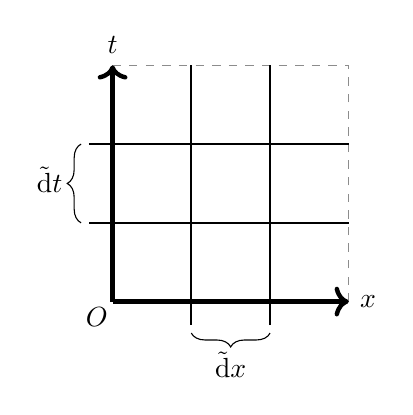
\begin{tikzpicture}
			\draw[help lines, color=gray!90, dashed] (0,0) grid (3,3);
			\draw[->,ultra thick] (0,0)--(3,0) node[right]{$x$};
			\draw[->,ultra thick] (0,0)--(0,3) node[above]{$t$};
			\draw[-, thick] (3,1)--(-0.3,1);
			\draw node at (-0.8, 1.55){$\tilde {\dd}t$};
			\draw[-, thick] (1,3)--(1,-0.3);
			\draw node at (1.5, -0.8){$\tilde {\dd}x$};
			\draw[-, thick] (-0.3,2)--(3,2);
			\draw[-, thick] (2,-0.3)--(2,3);
			\draw node at (-0.2,-0.2){$O$};	
			\draw [decorate,decoration={brace,amplitude=5pt}] (2,-0.4) -- (1,-0.4);
			\draw [decorate,decoration={brace,amplitude=5pt}] (-0.4,1) -- (-0.4,2);
		\end{tikzpicture}
	\end{center}

	\item \emph{Isotherms of a metal plate using one-forms.}
	Following the hint, For $\mathcal{P}$ we see that the basis vectors ${\vb e}_x$ and ${\vb e}_y$ cross the 0 and 2 surfaces respectively with respect to the origin, making the components of the gradient $\tilde {\dd}T \longrightarrow (-1,-1.5)$.

	\item \emph{Transformations as partial derivatives.}
	\begin{subquests}
		\item
		Transforming the vector coordinates to the frame $\bar O, \{x^{\bar \alpha}\}$ and back, the coordinate transformation is:
		\begin{gather*}
			x^{\alpha} = \pdv{x^{\alpha}}{x^{\bar\alpha}} \pdv{x^{\bar\alpha}}{x^{\beta}} x^{\beta}
		\end{gather*}
		We know from the chain rule that:
		\begin{gather*}
		 	\pdv{x^{\alpha}}{x^{\beta}} = \pdv{x^{\alpha}}{x^{\bar\alpha}} \pdv{x^{\bar\alpha}}{x^{\beta}}
		\end{gather*} 
		Since the components are just numbers in the same frame, we get the result:
		\begin{gather*}
			\pdv{x^{\alpha}}{x^{\beta}} = \delta^{\alpha}_{\;\;\beta}
		\end{gather*}
		
		\item Trivial extension.
	\end{subquests}

	\item \emph{Derivative notation.}
	3.14:
	\begin{gather*}
	 	\dv{\phi}{\tau} = \phi_{,\alpha}U^{\alpha} 
	\end{gather*} 
	3.15: This requires the one-form basis $\{\tilde \omega^{\alpha}\}$
	\begin{gather*}
	 	\tilde{\dd}\phi = \phi_{,\alpha}\tilde \omega^{\alpha} 
	\end{gather*} 
	3.18:
	\begin{gather*}
	 	x^{\beta}_{\;\;,\bar\alpha} = \Lambda^{\beta}_{\;\;\bar\alpha} \implies	\frac{\phi_{,\bar\alpha}}{\phi_{,\beta}} =\Lambda^{\beta}_{\;\;\bar\alpha} 
	\end{gather*} 
	A much more compact way of writing and understanding tensor expressions. Just keep track of the indices and find the respective partial derivatives!

	\item \emph{Normal one-forms.}
	\begin{subquests}
		\item
		This follows from the definition of a normal one-form: A one-form is said to be normal to a surface if its value is zero on every vector tangent to the surface. By inverting and negating both sides of the statement, we get: If the vector $\vec V$ is not tangent to the surface, then $\tilde n(\vec V) = 0$.

		\item		
		$\tilde n(\vec V) = n_{\alpha}V^{\alpha} > 0$, which means that the corresponding components of the one-form and vector are of the same sign. Any vector $\vec W$ having corresponding components with the same signs as those of $\vec V$ will result in $\tilde n(\vec W) > 0 $ because like signs multiplied result in positive numbers.

		\item		
		Consider a different normal one-form $\tilde p$ to S. Since S is the two-dimensional plane $x = 0$ (the y-z plane, essentially), $\tilde p$'s components in the standard one-form basis are $(p_x, 0, 0)$ and $\tilde n$'s components are $(n_x, 0, 0)$, so they are multiples of each other.

		\item
	\end{subquests}

	\item \emph{One-forms and surfaces.}
	Let $X$ be the surface of constant $f$. We take an object at point $A$ and displace it along $f$. From the property of one-forms:
	\begin{gather*}
		\tilde{\dd}f = \pdv{f}{x^{\alpha}} \tilde{\dd}x^{\alpha}
	\end{gather*}
	The change in $f$ with respect to any of the coordinates is 0, so any locally `tangential' movement along the surface results in no change of the one-form $\tilde{\dd}f$, indicating that only movements normal to the surface are registered by the property.

	\item \emph{Tensor product of one-forms.}
	Let $\vec A = (1, 0, 1, 0)$ and $\vec B = (1, -1, 0, 0)$. The tensors $\tilde p \otimes \tilde q$ and $\tilde q \otimes \tilde p$ are multi-linear maps that take two vectors as arguments and output the real numbers as follows:
	\begin{gather*}
		\tilde p (\vec A) \tilde q (\vec B) = p_{\alpha} A^{\alpha} q_{\beta} B^{\beta} = 1 \times -1 = -1 \\
		\tilde q (\vec A) \tilde p (\vec B) = q_{\alpha} A^{\alpha} p_{\beta} B^{\beta} = (-1 + 1) \times (1 - 1) = 0
	\end{gather*}
	The 16 components of $\tilde p \otimes \tilde q$ are found by feeding them the basis vectors $\tilde p(\vec e_{\alpha}) \tilde q (\vec e_{\beta})= p_{\alpha} q_{\beta}$. These components can be arranged into the $4\times 4$ matrix:
	\begin{gather*}
		\mqty[
			-1 & 0 & 1 & 0 \\
			-1 & 0 & 1 & 0 \\
			0 & 0 & 0 & 0 \\
			0 & 0 & 0 & 0
		]
	\end{gather*}

	\item \emph{Tensor basis.}
	The tensor ${\vb f} = f_{\alpha\beta} \tilde \omega^{\alpha\beta}$ must follow tensor transformation properties. So, when fed with basis vectors $(\vec e_{\mu}, \vec e_{\nu})$, we must get the components $f_{\mu\nu}$. The main question left to be answered is the description of $\omega^{\alpha\beta}$, which seems to be a basis `two-form' that takes in the previously mentioned basis vectors and transforms the components $f_{\alpha\beta}$ into $f_{\mu\nu}$.

	\item \emph{Symmetric and anti-symmetric tensors.}
	\begin{subquests}
		\item
		The definition of a symmetric tensor is: ${\vb f}(\vec A, \vec B) = {\vb f}(\vec B, \vec A), \forall \; \vec A, \vec B$. Therefore, all we have to check is if ${\vb h}_{(S)}(\vec A, \vec B) = {\vb h}_{(S)}(\vec B, \vec A)$. Following the definition, we get:
		\begin{gather*}
			{\vb h}_{(S)}(\vec A, \vec B) = \frac{1}{2}{\vb h}(\vec A, \vec B) + \frac{1}{2}{\vb h}(\vec B, \vec A)
			{\vb h}_{(S)}(\vec B, \vec A) = \frac{1}{2}{\vb h}(\vec B, \vec A) + \frac{1}{2}{\vb h}(\vec A, \vec B)
		\end{gather*}
		Which are indeed equal and satisfy the definition.

		\item		
		Switching the input vectors:
		\begin{gather*}
			{\vb h}_{(A)}(\vec B, \vec A) = \frac{1}{2}{\vb h}(\vec B, \vec A) - \frac{1}{2}{\vb h}(\vec A, \vec B) = -{\vb h}_{(A)}(\vec A, \vec B)
		\end{gather*}
		Which is indeed antisymmetric.

		\item		
		Let ${\vb h} = \tilde p \otimes \tilde q$. Then:
		\begin{gather*}
			{\vb h}_{(s)} =			
		\end{gather*}
		
		\item
		From the definition:
		\begin{gather*}
			{\vb h}_{(A)}(\vec A, \vec A) = \frac{1}{2}{\vb h}(\vec A, \vec A) - \frac{1}{2}{\vb h}(\vec A, \vec A) = 0
		\end{gather*}

		\item $\vb{h}_{(S)}$ and $\vb{h}_{(A)}$ have 10 independent and 6 components respectively.
	\end{subquests}

	\item \emph{Specific tensors.}
	\begin{subquests}
		\item
		A tensor that takes two vector arguments must consist of two one-forms taking the arguments, and is expressible in the form:
		\begin{gather*}
			{\vb h}(\;\;,\vec A) = \tilde{p}(\;\;)\tilde{q}(\vec A)
		\end{gather*}
		The objects $\tilde{p}(\vec A) = \beta_{A}$ and $\tilde{q}(\vec B) = \beta_B$ must be one-form expressions via proof:
		\begin{gather*}
			\gamma \tilde{p}(\vec A) = \frac{something}{darkside} 	
		\end{gather*}

		\item Show linearity.
	\end{subquests}

	\item \emph{Metric tensor as a mapping.}
	\begin{subquests}
		\item
		The one-form components can be found from the metric: $V_{\alpha} = g_{\alpha\beta}V^{\beta}$, which is simply inverting the sign of the time component. Therefore, the one-forms are:
		\begin{gather*}
			\tilde A \stackrel{O}\longrightarrow (-1, 0, 1, 0) \\
			\tilde B \stackrel{O}\longrightarrow (0, 1, 1, 0) \\
			\tilde C \stackrel{O}\longrightarrow (1, 0, -1, 0) \\
			\tilde D \stackrel{O}\longrightarrow (0, 0, 1, 1) 
		\end{gather*}
		
		\item The vector components can be found from the metric mapping: $V^{\alpha} = g^{\alpha\beta}V_{\beta}$, which is simply inverting the sign of the time component again. Therefore, the vectors are:
		\begin{gather*}
			\vec p \stackrel{O}\longrightarrow (-3, 0, -1, -1)^T \\
			\vec q \stackrel{O}\longrightarrow (-1, -1, 1, 1)^T \\
			\vec r \stackrel{O}\longrightarrow (0, -5→, -1, 0)^T \\
			\vec s \stackrel{O}\longrightarrow (2, 1, 0, 0)^T
		\end{gather*}
	\end{subquests}

	\item \emph{Metric tensor and scalar product of one-forms.}
	\begin{subquests}
		\item
		\begin{gather*}
			\eta^{\alpha\beta}\eta_{\beta\gamma} =
			\mqty[
				-1 & 0 & 0 & 0 \\
				0 & 1 & 0 & 0 \\
				0 & 0 & 1 & 0 \\
				0 & 0 & 0 & 1 
			]
			\mqty[
				-1 & 0 & 0 & 0 \\
				0 & 1 & 0 & 0 \\
				0 & 0 & 1 & 0 \\
				0 & 0 & 0 & 1
			]
			= 
			\mqty[
				1 & 0 & 0 & 0 \\
				0 & 1 & 0 & 0 \\
				0 & 0 & 1 & 0 \\
				0 & 0 & 0 & 1
			] = \delta^{\alpha}_{\gamma}
		\end{gather*}
		

		\item 	
		Transforming $\tilde q$ into a vector $\vec Q$ by using the metric tensor and feeding it to $\tilde p(\;)$:
		\begin{gather*}
			q^{\alpha} = g^{\alpha\beta}q_{\beta} \longrightarrow \vec Q \stackrel{O}\longrightarrow (-q_0, q_1, q_2, q_3) \\
			\tilde p \cdot \tilde q = \tilde p(\vec Q) = -p_0 q_0 + p_1 q_1 + p_2 q_2 + p_3 q_3
		\end{gather*}
	\end{subquests}

	\item \emph{Linear transformations.}
	\begin{subquests}
		\item
		The inverse of the matrix $\{\Lambda^{\bar \alpha}_{\;\;\beta}\}$ is $\{\Lambda^{\beta}_{\;\;\bar\alpha}\}$ from $V^{\beta} = \Lambda^{\beta}_{\;\;\bar\alpha}V^{\bar\alpha}$. Its transpose is simply found by switching the index positions and switching the frames: $\{\Lambda^{\alpha}_{\;\;\bar\beta}\}$. This is the transformation matrix we've seen for one-form components: $P_{\bar\beta} = \Lambda^{\alpha}_{\;\;\bar\beta}P_{\alpha}$.

		\item
	\end{subquests}

	\item \emph{One-forms and vectors in spacetime diagrams.}
	\begin{subquests}
		\item
		The situation described is:
		\begin{center}
			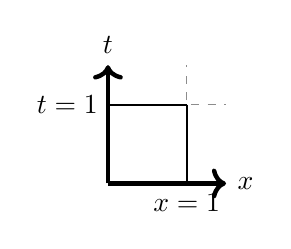
\begin{tikzpicture}
				\draw[help lines, color=gray!90, dashed] (0,0) grid (1.5,1.5);
				\draw[->,ultra thick] (0,0)--(1.5,0) node[right]{$x$};
				\draw[->,ultra thick] (0,0)--(0,1.5) node[above]{$t$};
				\draw[-, thick] (1,1)--(1,0) node[below]{$x=1$};
				\draw[-, thick] (1,1)--(0,1) node[left]{$t=1$};
			\end{tikzpicture}
		\end{center}
		The outward normal one-forms and their associated vectors are:
		\begin{gather*}
			t = 0 \rightarrow -\tilde{\dd}t, \;\; t = 1 \rightarrow \tilde{\dd}t, \;\; x = 0 \rightarrow -\tilde{\dd}x, \;\; x = 1 \rightarrow \tilde{\dd}x \\
			-V^0(t = 0), \;\; V^0(t = 1), \;\; -V^1(x = 0), \;\; V^1(x = 1)
		\end{gather*}
		
		\item		
		The situation described is:
		\begin{center}
			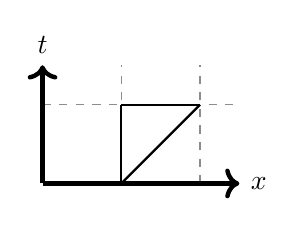
\begin{tikzpicture}
				\draw[help lines, color=gray!90, dashed] (0,0) grid (2.5,1.5);
				\draw[->,ultra thick] (0,0)--(2.5,0) node[right]{$x$};
				\draw[->,ultra thick] (0,0)--(0,1.5) node[above]{$t$};
				\draw[-, thick] (1,0)--(1,1);
				\draw[-, thick] (1,1)--(2,1);
				\draw[-, thick] (2,1)--(1,0);
			\end{tikzpicture}
		\end{center}
	\end{subquests}

	\item \emph{Duality of one-forms and vectors.} Trivial.

	\item \emph{Tensors as a vector space.}
	\begin{subquests}
		\item
		Let $A$ be the set of all $\pmqty{M \\ N}$ tensors for fixed $M, N \in \mathcal{R}$, e.g. an element in $A$ is \\
		${\vb T}(\underbrace{\vec A, \vec B, \vec C, \vec D, ...}_{M\;vectors};\underbrace{\tilde T,\tilde U, \tilde V, \tilde W, ...}_{N\;one-forms})$. The addition of two tensors of the same rank and multiplication of tensors by numbers are defined as:
		\begin{gather*}
			{\vb T}(\;) = {\vb R}(\;) + {\vb S}(\;) \\
			{\vb P}(\;) = \alpha {\vb Q}(\;)   
		\end{gather*}
		This description is consistent with the defined set: It is closed under addition and scalar multiplication. The addition of these tensors is a commutative operation because the tensors are all fed the same arguments.
	
		\item	
	\end{subquests}

	\item {Playing with rank-two tensors.}
	\begin{subquests}
		\item
		\begin{subquests}
			\item
			\begin{gather*}
				M^{\pqty{\alpha \beta}} = \frac{1}{2}\pqty{M^{\alpha \beta} + M^{\beta \alpha}} = \frac{1}{2} \pqty{
				\mqty[
					0 & 1 & 0 & 0 \\
					1 & -1 & 0 & 2 \\
					2 & 0 & 0 & 1 \\
					1 & 0 & -2 & 0
				]
				+
				\mqty[
					0 & 1 & 2 & 1 \\
					1 & -1 & 0 & 0 \\
					0 & 0 & 0 & -2 \\
					0 & 2 & 1 & 0 \\
				]} \\
				= \frac{1}{2}
				\mqty[
					0 & 2 & 2 & 1 \\
					2 & -2 & 0 & 2 \\
					2 & 0 & 0 & -1 \\
					1 & 2 & -1 & 0
				] \\
				M^{\bqty{\alpha \beta}} = \frac{1}{2}\pqty{M^{\alpha \beta} - M^{\beta \alpha}} = \frac{1}{2} \pqty{
				\mqty[
					0 & 1 & 0 & 0 \\
					1 & -1 & 0 & 2 \\
					2 & 0 & 0 & 1 \\
					1 & 0 & -2 & 0
				]
				-
				\mqty[
					0 & 1 & 2 & 1 \\
					1 & -1 & 0 & 0 \\
					0 & 0 & 0 & -2 \\
					0 & 2 & 1 & 0 \\
				]} \\
				= \frac{1}{2}
				\mqty[
					0 & 0 & -2 & -1 \\
					0 & 0 & 0 & 2 \\
					2 & 0 & 0 & 1 \\
					1 & -2 & -3 & 0
				]
			\end{gather*}
			
			\item
			Lowering the index using the metric tensor:
			\begin{gather*}
				M^{\alpha}_{\;\;\beta} = g_{\mu \beta} M^{\alpha \mu} =
				\mqty[
					-1 & 0 & 0 & 0 \\
					0 & 1 & 0 & 0 \\
					0 & 0 & 1 & 0 \\
					0 & 0 & 0 & 1
				]
				\mqty[
					0 & 1 & 0 & 0 \\
					1 & -1 & 0 & 2 \\
					2 & 0 & 0 & 1 \\
					1 & 0 & -2 & 0
				]\\
				=
				\mqty[
					0 & -1 & 0 & 0 \\
					1 & -1 & 0 & 2 \\
					2 & 0 & 0 & 1 \\
					1 & 0 & -2 & 0
				]
			\end{gather*}
			
			\item
			Lowering the other index:
			\begin{gather*}
				M_{\alpha}^{\;\;\beta} = g_{\alpha \mu} M^{\mu \beta} =
				\mqty[
					-1 & 0 & 0 & 0 \\
					0 & 1 & 0 & 0 \\
					0 & 0 & 1 & 0 \\
					0 & 0 & 0 & 1
				]
				\mqty[
					0 & 1 & 0 & 0 \\
					1 & -1 & 0 & 2 \\
					2 & 0 & 0 & 1 \\
					1 & 0 & -2 & 0
				]\\
				=
				\mqty[
					0 & 1 & 0 & 0 \\
					-1 & -1 & 0 & 2 \\
					-2 & 0 & 0 & 1 \\
					-1 & 0 & -2 & 0
				]
			\end{gather*}
			
			\item
			Lowering the $\pmqty{1 \\ 1}$ tensor index:
			\begin{gather*}
				M_{\alpha \beta} = g_{\mu \beta} M_{\alpha}^{\;\;\mu} =
				\mqty[
					-1 & 0 & 0 & 0 \\
					0 & 1 & 0 & 0 \\
					0 & 0 & 1 & 0 \\
					0 & 0 & 0 & 1
				]
				\mqty[
					0 & 1 & 0 & 0 \\
					-1 & -1 & 0 & 2 \\
					-2 & 0 & 0 & 1 \\
					-1 & 0 & -2 & 0
				] \\
				= 
				\mqty[
					0 & 1 & 0 & 0 \\
					1 & -1 & 0 & 2 \\
					2 & 0 & 0 & 1 \\
					1 & 0 & -2 & 0
				]
			\end{gather*}
		\end{subquests}

		\item Yes, but defining it would take time.

		\item Trivial.
	\end{subquests}

	\item \emph{Contraction of tensors.} This is a double summation over the tensor components, which results in a scalar.

	\item \emph{Products of symmetric and anti-symmetric tensors.}
	\begin{subquests}
		\item

		\item

		\item
	\end{subquests}

	\item \emph{Raising and lowering indices.}
	\begin{subquests}
		\item 

		\item
	\end{subquests}

	\item \emph{Derivative of a tensor.}
	Notice the following about the expression:
	\begin{gather*}
		\dv{{\vb T}}{\tau} = (T^{\alpha}_{\;\;\beta,\gamma}{\tilde \omega}^\beta \otimes {\vec e}_{\alpha})U^{\gamma} = \pdv{T^{\alpha}_{\;\;\beta}}{x^{\gamma}}\dv{x^{\gamma}}{\tau} \\
		\dd{{\vb T}} =  (T^{\alpha}_{\;\;\beta,\gamma}{\tilde \omega}^\beta \otimes {\vec e}_{\alpha})\dd{x}^{\gamma} = \nabla{\vb T}\pqty{\dd{\vec s}}
	\end{gather*}
	For $\nabla{\vb T}$ to be a legitimate tensor, there must exist a basis one-form $\tilde \omega^{\gamma}$ for the $\gamma$ component, giving:
	\begin{gather*}
		\nabla{\vb T} = T^{\alpha}_{\;\;\beta,\gamma}{\tilde \omega}^{\beta} \otimes {\tilde \omega}^{\gamma} \otimes {\vec e}_{\alpha}
	\end{gather*}
	Evidently the gradient of $\vb T$ is a $\pmqty{1 \\ 2}$ tensor.

	\item \emph{Leibniz rule for tensors.}

	\item \emph{Practice with tensors.}
	\begin{subquests}
		\item
		\begin{gather*}
			\vec U \cdot \vec U = -(1+t^2)^2 + (t^2)^2 + (\sqrt{2} t)^2 = -1 \\
			\vec U \cdot \vec D = -(1+t)x + 5xt^3 + 2t^2 =  \\
			\vec D \cdot \vec D = -x^2 + 25t^2 x^2 + 2t^2 \\
		\end{gather*}
		$\vec U$ is suitable, but $\vec D$ is not. 

		\item		
		The spatial velocity is:
		\begin{gather*}
		 	{\va v} = \frac{t^2}{1+t^2}{\va e}_x + \frac{\sqrt{2}t}{1+t^2}{\va e}_y \\
		 	{\va v}_{t\to 0} = {\va 0} \\
		 	{\va v}_{t \to \infty} = {\va e}_x
		\end{gather*} 

		\item		
		This is the same as finding the one-form components: ${\tilde U} \longrightarrow (-(1+t)^2, t^2, \sqrt{2}t, 0)$ 

		\item		
		This is differentiation of the components with respect to each coordinate. Since there is only a time dependence, the derivatives with respect to the spatial coordinates are zero.
		\begin{gather*}
			U^t_{\;\;,t} = \pdv{U^t}{t} = 2t, \;\; U^x_{\;\;,t} = \pdv{U^x}{t} = 2t, \;\; U^y_{\;\;,t} = \sqrt{2}, \;\; U^z_{\;\;,t} = 0
		\end{gather*}

		\item		
		Evaluating the expressions:
		\begin{gather*}
			U_{\alpha}U^{\alpha}_{\;\;,t} = U_{t}U^{t}_{\;\;,t} + U_{x}U^{x}_{\;\;,t} + U_{y}U^{y}_{\;\;,t} + U_{z}U^{z}_{\;\;,t} = -(1+t^2)\times 2t + 2t^3 + 2t = 0 
		\end{gather*}

		\item		
		\begin{gather*}
			D^{\beta}_{\;\;,\beta} = D^{t}_{\;\;,t} + D^{x}_{\;\;,x} + D^{y}_{\;\;,y} + D^{z}_{\;\;,z} = 5t 
		\end{gather*}
		\item

		\item

		\item		
		Performing the required differentiation and using the metric tensor to raise the index:
		\begin{gather*}
			\rho_{,t} = 2t, \;\; \rho_{,x} = 2x, \;\; \rho_{,y} = -2y, \;\; \rho_{,z} = 0 \\
			\rho^{,t} = -2t, \;\; \rho^{,x} = 2x, \;\; \rho^{,y} = -2y, \;\; \rho^{,z} = 0
		\end{gather*}
		The numbers $\rho^{,\alpha}$ are the components of the vector gradient. 

		\item		
		The expressions are evaluated:
		\begin{gather*}
			\nabla_{\vec U }\rho = \rho_{,\gamma}U^{\gamma} = 2t(1+t^2) + 2x(t^2) - 2y(\sqrt{2}t) \\
			\nabla_{\vec U}\vec{D} = D^{\alpha}_{\;\;,\gamma}U^{\gamma} \longrightarrow (t^2, 5x + 5xt^2 + 5t^3, 2t, 0)\\
			\nabla_{\vec D}\rho = \rho_{,\gamma}D^{\gamma} = 2t(x) + 2x(5tx) - 2y(\sqrt{2}t)\\
			\nabla_{\vec D}\vec{U} = U^{\beta}_{\;\;,\gamma}D^{\gamma} \longrightarrow (2tx, 10 t^2 x^2, 2t, 0)
		\end{gather*}
	
	\end{subquests}

	\item \emph{Projection tensor.}
	\begin{subquests}
		\item
		\begin{subquests}
			\item
			The following computation yields:
			\begin{gather*}
				\vec{U}\cdot\vec{V}_{\perp} = \vec{U}(\tilde{V}_{\perp}) = U_{\alpha} V^{\alpha}_{\perp} = U_{\alpha}\pqty{\eta^{\alpha}_{\;\;\beta} + U^{\alpha} U_{\beta}}V^{\beta} \\
				= U_{\beta} V^{\beta} + U_{\alpha} U^{\alpha} U_{\beta} V^{\beta} = U_{\alpha} V^{\beta} - U_{\alpha} V^{\beta} = 0,
			\end{gather*}
			
			\item
			Performing the operation ${\vb P}\vec{V}_{\perp}$:
			\begin{gather*}
				V^{\alpha}_{\perp\perp} = P^{\alpha}_{\;\;\beta} P^{\beta}_{\;\;\mu} V^{\mu} = \pqty{\eta^{\alpha}_{\;\;\beta} + U^{\alpha}U_{\beta}}\pqty{\eta^{\beta}_{\;\;\mu} + U^{\beta}U_{\mu}}V^{\mu}\\ = \pqty{\delta^{\alpha}_{\mu} - U^{\alpha} U_{\mu} + 2U^{\alpha} U_{\mu}}V^{\mu}  
				= \pqty{\delta^{\alpha}_{\;\;\mu} + U^{\alpha} U_{\mu}}V^{\mu} = V^{\alpha}_{\perp}	
			\end{gather*}
		\end{subquests}

		\item
		The corresponding vector $\vec{q}_{\perp}$ is:
		\begin{gather*}
			q^{\mu}_{\perp} = \pqty{\eta^{\mu}_{\;\;\nu} - \frac{q^{\mu}q_{\nu}}{q^{\alpha} q_{\alpha}}} q^{\nu} \\
			\vec{q}\cdot\vec{q}_{\perp} = q_{\mu} q^{\mu}_{\perp} = q_{\mu}\pqty{\eta^{\mu}_{\;\;\nu} - \frac{q^{\mu}q_{\nu}}{q^{\alpha} q_{\alpha}}} q^{\nu} = 0
		\end{gather*}
		If $\vec{q}$ is null, $q_{\alpha} q^{\alpha} = 0$ and therefore the expression is invalid. Thus, $\vb P$ is restricted to non-null unit vectors satisfying $U_{\alpha} U^{\alpha} = -1$.

		\item		
		Feeding the vectors to the tensor:
		\begin{gather*}
			{\vb P}(\vec{V}_{\perp},\vec{W}_{\perp}) = P_{\mu\nu} V^{\mu}_{\perp} W^{\nu}_{\perp} = \pqty{\eta_{\mu\nu} + U_{\mu} U_{\nu}}\pqty{\eta^{\mu}_{\;\;\alpha} + U^{\mu} U_{\alpha}}\pqty{\eta^{\nu}_{\;\;\beta} + U^{\nu} U_{\beta}} V^{\alpha} W^{\beta} \\
			= \eta_{\mu\nu} \eta^{\mu}_{\;\;\alpha} \eta^{\nu}_{\;\;\beta} + U_{\mu} U_{\nu} U^{\mu} U_{\alpha} U^{\nu} U_{\beta}
		\end{gather*}
	\end{subquests}

	\item \emph{Tensor transformations as matrices.}

	\item \emph{The Lorentz group.}

	\item \emph{Tensors in Minkowski space.}
	\begin{subquests}
		\item
		\begin{gather*}
			t = \frac{u + v}{2}, \;\; x = \frac{v - u}{2} \\
			u = 1, \;\; v = 1 \longrightarrow t = 1, \;\; x = 0 \longrightarrow \vec{e}_t = \frac{\vec{e}_u + \vec{e}_v}{2} \\
			u = -1, \;\; v = 1 \longrightarrow t = 0, \;\; x = 1 \longrightarrow \vec{e}_x = \frac{\vec{e}_v - \vec{e}_u}{2} \\
			\vec{e}_u = \frac{\vec{e}_t - \vec{e}_x}{2}, \;\; \vec{e}_v = \frac{\vec{e}_t + \vec{e}_x}{2}		
		\end{gather*}
		\begin{center}
			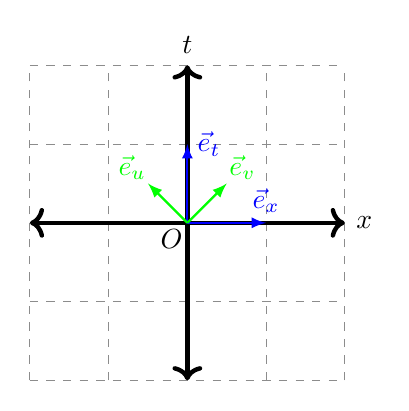
\begin{tikzpicture}
				\draw[help lines, color=gray!90, dashed] (-2,-2) grid (2,2);
				\draw[<->,ultra thick] (-2,0)--(2,0) node[right]{$x$};
				\draw[<->,ultra thick] (0,-2)--(0,2) node[above]{$t$};
				\draw node at (-0.2,-0.2){$O$};
				\draw[-latex, blue, thick] (0,0) -- (1,0) node[above]{$\vec{e}_x$};
				\draw[-latex, blue, thick] (0,0) -- (0,1) node[right]{$\vec{e}_t$};
				\draw[-latex, green, thick] (0,0) -- (-0.5,0.5) node at (-0.7,0.7){$\vec{e}_u$};
				\draw[-latex, green, thick] (0,0) -- (0.5,0.5) node at (0.7,0.7){$\vec{e}_v$};
			\end{tikzpicture}
		\end{center}

		\item
		The matrix formed by the basis vectors form the identity matrix, with a non-zero determinant. Clearly the set of vectors are linearly independent and span Minkowski space,	thus form a basis.

		\item
		By evaluating the dot products of the basis vectors $\vec{e}_{\mu} \cdot \vec{e}_{\nu}$, we find the matrix representing the metric tensor:
		\begin{gather*}
			g_{\mu\nu} = {\vb g}\pqty{\vec{e}_{\mu},\vec{e}_{\nu}} =
			\mqty[
				0 & -1/2 & 0 & 0 \\
				-1/2 & 0 & 0 & 0 \\
				0 & 0 & 1 & 0 \\
				0 & 0 & 0 & 1			
			]
		\end{gather*}

		\item
		This is evident from the dot product calculations of the previous part.

		\item
		The one-forms are simply found by evaluating the differential forms and substituting. ${\vb g}(\vec{e}_u,\;\;)$ are the basis one-forms in the u-v plane, which is simply inverting the sign of the time component of the basis vectors by the metric tensor. 
		\begin{gather*}
			\tilde{\dd}u = \tilde{\dd}t - \tilde{\dd}x, \;\; \tilde{\dd}v = \tilde{\dd}x + \tilde{\dd}t	\\
			{\vb g}\pqty{\vec{e}_u, \;\;} = -\frac{\tilde{\dd}v}{2} = - \frac{1}{2}\tilde{\dd}t - \frac{1}{2}\tilde{\dd}x, \;\; {\vb g}\pqty{\vec{e}_u, \;\;} = - \frac{\tilde{\dd}u}{2} = -\frac{1}{2}\tilde{\dd}t + \frac{1}{2}\tilde{\dd}x
		\end{gather*}
	\end{subquests}
\end{subquests}

\chapter{Perfect fluids in special relativity}

\begin{subquests}
	\item \emph{The continuum approximation.}
	\begin{subquests}
		\item 
		No, the objects are too far apart and too unalike.

		\item
		Yes, the medium can be considered as homogeneous.

		\item
		Yes, because the traffic is moving very slowly and is in large numbers close together.

		\item
		No, because the traffic motion isn't homogeneous.

		\item
		Yes, the continuum approximation suits plasma because it is homogeneous.
	\end{subquests}

	\item \emph{Terminology of flux.}

	\item \emph{Galilean momentum.}
	\begin{subquests}
		\item

		\item
	\end{subquests}

	\item \emph{Number density of dust.}
	$\vec{N}\cdot\vec{N} = n^2\vec{U}\cdot\vec{U} = -n^2$.

	\item {Definition of tensor as a bilinear object.}
	\begin{gather*}
		{\vb T}\pqty{a\tilde{\dd}x^{\alpha} + b\tilde{\dd}x^{\mu}, \tilde{\dd}x^{\beta}} = a{\vb T}\pqty{\tilde{\dd}x^{\alpha}, \tilde{\dd}x^{\beta}} + b{\vb T}\pqty{\tilde{\dd}x^{\mu}, \tilde{\dd}x^{\beta}} = a T^{\alpha\beta} + b T^{\mu\beta}\\
		{\vb T}\pqty{\tilde{\dd}x^{\alpha}, a\tilde{\dd}x^{\beta} + b\tilde{\dd}x^{\mu}} = a{\vb T}\pqty{\tilde{\dd}x^{\alpha}, \tilde{\dd}x^{\beta}} + b{\vb T}\pqty{\tilde{\dd}x^{\alpha}, \tilde{\dd}x^{\mu}} = a T^{\alpha\beta} + b T^{\alpha\mu}
	\end{gather*}

	\item \emph{Definition of dust.}
	\begin{gather*}
			\vb T = T^{\alpha\beta} \vec{e}_{\alpha} \otimes \vec{e}_{\beta}
		\end{gather*}
		Since $T^{00} = \rho$ and the other components are zero in the MCRF, we can express it as a product of the number-flux four-vector and the four-momentum in the MCRF, because $\vec{N} \stackrel{MCRF}\longrightarrow (n, 0, 0, 0)$ and $\vec{p} \stackrel{MCRF}\longrightarrow (m, 0, 0, 0)$:
		\begin{gather*}
			\vb T = \vec{p} \otimes \vec{N}
		\end{gather*}

	\item \emph{Stress-energy tensor of dust.}
	This can be deduced by applying a Lorentz transformation from the frame $O$ to $\bar O$:
	\begin{gather*}
		T^{\bar \alpha \bar \beta} = \Lambda^{\bar \alpha}_{\;\;\alpha}\Lambda^{\bar \beta}_{\;\;\beta} T^{\alpha\beta} = \rho \Lambda^{\bar \alpha}_{\;\;\alpha}\Lambda^{\bar \beta}_{\;\;\beta} U^{\alpha} U^{\beta} \longrightarrow \pqty{\bar T} = \rho\pqty{\Lambda^T}\pqty{\vec U \otimes \vec U}\pqty{\Lambda}
	\end{gather*}

	\item \emph{Thermodynamic relations as one-forms.}

	\item \emph{Newton's second law from the stress-energy tensor.}
	The expression is $T^{i\beta}_{\;\;\;,\beta} = 0, \quad i = 1,2,3$. $T^{i0}$ corresponds to the momentum density, $T^{ij}$ corresponds to the flux of $i$ momentum across $j$ surface. Expanding:
	\begin{gather*}
		T^{i0}_{\;,0} + T^{ix}_{\;,x} + T^{iy}_{\;,y} + T^{iz}_{\;,z} = 0 \\
		\int_{V} \div{T^i}\,\dd{V} = -\int_V T^{i0}_{\;,0}\,\dd{V}
	\end{gather*}
	and thus this expression indicates the divergence of the momentum density across the space-time coordinates.

	\item \emph{Continuity equation of number flux four-vector.}
	\begin{gather*}
		N^{\alpha}_{\;,\alpha} = \pqty{nU^{\alpha}}_{\;,\alpha} = (n\gamma)_{,t} + (n\gamma v^x)_{,x} + (n\gamma v^y)_{,y} + (n\gamma v^z)_{,z} \\
		 \approx n_{,t} + (nv^x)_{,x} + (nv^y)_{,y} + (nv^z)_{,z} = 0
	\end{gather*}

	\item \emph{Transformation of Kronecker delta.}
	\begin{subquests}
		\item

		\item
	\end{subquests}

	\item \emph{Tensorial form of perfect fluids.}
	\begin{gather*}
		T^{\alpha\beta} = 
		\mqty[
			\rho + p & 0 & 0 & 0 \\
		 	0 & 0 & 0 & 0 \\
		 	0 & 0 & 0 & 0 \\
		 	0 & 0 & 0 & 0
		 	]
		+
		\mqty[
			-p & 0 & 0 & 0 \\
			0 & p & 0 & 0 \\
			0 & 0 & p & 0 \\
			0 & 0 & 0 & p
			]
	\end{gather*}
	In the MCRF $\vec{U} = \vec{e}_0$. Therefore $\vec U \otimes \vec U$ in the MCRF is a matrix with the first entry 1 and all other entries as zero. The second matrix is $p$ multiplied by the metric tensor, giving:
	\begin{gather*}
		T^{\alpha\beta} = \pqty{\rho + p}U^{\alpha}U^{\beta} + p\eta^{\alpha\beta}
	\end{gather*}

	\item \emph{Derivative of a dot product.}
	The metric tensor in Minkowski spacetime has only constants, so there are no derivatives. The indices $\alpha$ and $\gamma$ can be interchanged, then using the symmetry of the metric tensor to arrive at the conclusion.

	\item \emph{Conservation of entropy in the MCRF.}
	In the MCRF, $\vec{U} = \vec{e}_0$, so all spatial terms vanish by its multiplication.

	\item \emph{More on conservation of entropy.}
	Trivial.

	\item \emph{Acceleration in the MCRF.}
	The three-velocity derivatives correspond to the local and convective acceleration, which may be non-zero in the MCRF. This is similar to the argument: $\dd(\sin x) \neq 0$ when $\sin x = 0$.

	\item \emph{Euler equation.}
	For the four-vector $\vec U \stackrel{O}\longrightarrow (U^t, U^x, U^y, U^z)$, evaluating the expression in the frame $O$ that is not the MCRF yields:
	\begin{gather*}
		a^{\mu} = U^{\mu}_{,\beta}U^{\beta} = \pdv{U^{\mu}}{x^{\beta}}U^{\beta} \\
		a^{i} = U^{i}_{,\beta}U^{\beta} = U^{i}_{,t}U^t + U^i_{,j}U^{j}
	\end{gather*}
	In the small-velocity approximation, the four-vector $\vec U \stackrel{O}\longrightarrow (1,v^x,v^y,v^z)$ is a reduction to the three-velocity ${\vb v}$. Therefore, $U^i_{,t}$ just denotes the time derivatives of the spatial velocity components, which is simply the three-acceleration $\dot{v}^i$. The rest of the terms describe the convective derivative $U^i_{,j}U^{j} = \pqty{{\vb v \cdot \nabla}}v^i$. The final expression is:
	\begin{gather*}
		a^i = \dot{v}^i + \pqty{{\vb v \cdot \nabla}}v^i = \frac{Dv^i}{Dt}
	\end{gather*}
	Which is just the Euler equation from fluid mechanics.

	\item \emph{Newton's law.}

	\item \emph{Gauss' theorem.}
	The difference between the coordinates $\bqty{V^t(t_2) - V^t(t_1)}$ is simply the differential change in time with respect to the time component of the four-vector multiplied by the time difference, expressible as $(\partial V^t/\partial t)\dd{t}$. Analogous arguments for the spatial displacements $\bqty{V^x(x_2) - V^x(x_1)}$ give the following expression:
	\begin{gather*}
		\int \pdv{V^t}{t} \dd{t}\dd{x}\dd{y}\dd{z} + \int \pdv{V^x}{x}\dd{x}\dd{t}\dd{y}\dd{z} + ... \\
		= \int \pdv{V^{\alpha}}{x^{\alpha}} \dd^4{x} = \int V^{\alpha}_{,\alpha} \dd^4{x}
	\end{gather*}
	This is simply the divergence of the vector through the four-volume, verifying Gauss' theorem.

	\item \emph{Non-conservative system.}
	\begin{subquests}
		\item

		\item
	\end{subquests}

	\item \emph{Practice with the stress-energy tensor.}
	\begin{subquests}
		\item

		\item

		\item
	\end{subquests}

	\item \emph{Photon gas.}

	\item \emph{Theorems from conservation of the stress-energy tensor.}
	\begin{subquests}
		\item

		\item

		\item
	\end{subquests}
	
	\item \emph{Astronomical radiation.}
	\begin{subquests}
		\item

		\item

		\item
	\end{subquests}
	
	\item \emph{Electromagnetism in special relativity.}
	\begin{subquests}
		\item
		Using the antisymmetry, the components of the electromagnetic field tensor $F^{\mu\nu}$	can be represented as the matrix:
		\begin{gather*}
			F^{\mu\nu} =
			\begin{bmatrix}
				0 & E^x & E^y & E^z \\
				-E^x & 0 & B^z & -B^y \\
				-E^y & -B^z & 0 & B^x \\
				-E^z & B^y & -B^x & 0
			\end{bmatrix}
		\end{gather*}
		
		\item		
		The transformation follows $\pqty{\bar F} = \pqty{\Lambda^T}\pqty{F}\pqty{\Lambda}$:
		\begin{gather*}
			F^{\alpha'\beta'} =
			\begin{bmatrix}
				1 & 0 & 0 & 0 \\
				0 & \cos\theta & \sin\theta & 0 \\
				0 & -\sin\theta & \cos\theta & 0 \\
				0 & 0 & 0 & 1
			\end{bmatrix}
			\begin{bmatrix}
				0 & E^x & E^y & E^z \\
				-E^x & 0 & B^z & -B^y \\
				-E^y & -B^z & 0 & B^x \\
				-E^z & B^y & -B^x & 0
			\end{bmatrix}
			\begin{bmatrix}
				1 & 0 & 0 & 0 \\
				0 & \cos\theta & -\sin\theta & 0 \\
				0 & \sin\theta & \cos\theta & 0 \\
				0 & 0 & 0 & 1
			\end{bmatrix} \\
			=
			\begin{bmatrix}
				1 & 0 & 0 & 0 \\
				0 & \cos\theta & \sin\theta & 0 \\
				0 & -\sin\theta & \cos\theta & 0 \\
				0 & 0 & 0 & 1
			\end{bmatrix}
			\begin{bmatrix}
				0 & E^x\cos\theta + E^y\sin\theta & -E^x\sin\theta + E^y\cos\theta & E^z \\
				-E^x & B^z\sin\theta  & B^z\cos\theta & -B^y \\
				-E^y & -B^z\cos\theta & B^z\sin\theta & B^x \\
				-E^z & B^y\cos\theta - B^x\sin\theta & -(B^y\sin\theta + B^x\cos\theta) & 0
			\end{bmatrix} \\
			=
			\begin{bmatrix}
				0 & E^x\cos\theta + E^y\sin\theta & E^y\sin\theta - E^x\sin\theta & E^z \\
				-(E^x\cos\theta + E^y\sin\theta) & 0 & B^z & B^x\sin\theta-B^y\cos\theta \\
				-(E^y\cos\theta - E^x\sin\theta) & -B^z & 0 & B^y\sin\theta + B^x\cos\theta \\
				-E^z & -(B^x\sin\theta-B^y\cos\theta) & -(B^y\sin\theta + B^x\cos\theta) & 0
			\end{bmatrix}
		\end{gather*}
		
		\item		
		The components are evaluated as follows:
		\begin{gather*}
			\div{{\vb E}} = 4\pi\rho \longrightarrow E^i_{,i} = 4\pi J^t = \bqty{F^{ti}_{,i}} \qq{and} \bqty{F^{tt}_{,t}} = 0 \longrightarrow F^{t\nu}_{,\nu} = 4\pi J^t \\
			(\curl{{\vb B}})_x - \pdv{E^x}{t} = \pqty{\pdv{B^z}{y} - \pdv{B^y}{z}} - \pdv{E^x}{t} = 4\pi J^x = \bqty{F^{x\nu}_{,\nu}}
		\end{gather*}
		The curl expression can be simplified using the Levi-Civita tensor and converting the magnetic field vector into a one-form. The final expression can then be obtained via combination:
		\begin{gather*}
			4\pi J^t = \bqty{F^{t\nu}_{,\nu}} \\
			\epsilon^{ijk}B_{j,k} - E^i_{\;\;,t} = 4\pi J^i = \bqty{F^{i\nu}_{,\nu}} \\
			\bqty{F^{\mu\nu}_{,\nu} = 4\pi J^{\mu}}
		\end{gather*}
		
		\item		
		Lowering indices of $F^{\mu\nu}$ using the metric tensor inverts the signs of all the components, giving its transpose:
		\begin{gather*}
			F_{\mu\nu} = g_{\mu\alpha}g_{\beta\nu} F^{\alpha\beta} =
			\begin{bmatrix}
				0 & -E^x & -E^y & -E^z \\
				E^x & 0 & -B^z & B^y \\
				E^y & B^z & 0 & -B^x \\
				E^z & -B^y & B^x & 0
			\end{bmatrix}
		\end{gather*}
		$F_{\mu\nu,\lambda}$ is a $\pmqty{0 \\ 3}$ tensor with 24 components consisting of all the derivatives of the electromagnetic field tensor. Now, evaluating the remaining Maxwell equations:
		\begin{gather*}
			\div{{\vb B}} = 0 \longrightarrow B^i_{\;\;,i} = 0 \\
			\epsilon^{ijk} E_{j,k} + B^i_{\;\;,t} = 0
		\end{gather*}

		\item

		\item

		\item

		\item
	\end{subquests}
\end{subquests}

% \begin{chapter4}\label{prob: 21}
	
% \end{chapter4}

% \begin{chapter4}\label{prob: 22}
	
% \end{chapter4}

% \begin{chapter4}\label{prob: 23}
	
% \end{chapter4}

% \begin{chapter4}\label{prob: 24}
	
% \end{chapter4}

% \begin{chapter4}\label{prob: 25}
% 
% 		\stepcounter{subpart4}
% 		
		
% 		
% \end{chapter4}

% \newtheorem{chapter5}{Problem}
% \newcounter{subpart5}[chapter5]
% \newcounter{subsubpart5}[chapter5]

% \chapter{Preface to Curvature}

% \begin{chapter5}\label{prob: 1}
	
% \end{chapter5}

% \begin{chapter5}\label{prob: 2}
% 	All objects would experience the same gravitational force in the same direction. This is analogous to free-fall.
% \end{chapter5}

% \begin{chapter5}\label{prob: 3}
% 
% 		\stepcounter{subpart5}
% 		
% 		\begin{gather*}
% 			\begin{vmatrix}
% 				\pdv{\xi}{x} & \pdv{\xi}{y} \\
% 				\pdv{\eta}{x} & \pdv{\eta}{y} 
% 			\end{vmatrix}
% 			=
% 			\begin{vmatrix}
% 				1 & 0 \\
% 				0 & 0 \\
% 			\end{vmatrix}
% 			= 0
% 		\end{gather*}
% 		\stepcounter{subpart5}
% 		
% 		\stepcounter{subsubpart5}
% 		(\roman{subsubpart5})
% 		\begin{gather*}
% 			\mqty|\pdv{\xi}{x} & \pdv{\xi}{y} \\ \pdv{\eta}{x} & \pdv{\eta}{y}| = \mqty|\frac{x}{\sqrt{x^2+y^2}} & \frac{y}{\sqrt{x^2 + y^2}} \\ -\frac{x}{\pqty{x^2 + y^2}} & \frac{y}{\pqty{x^2 + y^2}}| = \frac{\pqty{xy}^2}{\pqty{x^2+y^2}^{3/2}} \neq 0
% 		\end{gather*}
% 		Fails at the origin. \\\\
% 		\stepcounter{subsubpart5}
% 		(\roman{subsubpart5})
% 		\begin{gather*}
% 			\mqty|\pdv{\xi}{x} & \pdv{\xi}{y} \\ \pdv{\eta}{x} & \pdv{\eta}{y}| = \mqty|1/x & 0 \\ 0 & 1| = \frac{1}{x} \neq 0  
% 		\end{gather*}
% 		Fails at $x \leq 0$. \\\\
% 		\stepcounter{subsubpart5}
% 		(\roman{subsubpart5})
% 		\begin{gather*}
% 			\mqty|\pdv{\xi}{x} & \pdv{\xi}{y} \\ \pdv{\eta}{x} & \pdv{\eta}{y}| = \mqty|-\frac{x}{\pqty{x^2 + y^2}} & \frac{y}{\pqty{x^2 + y^2}} \\ -\frac{3x}{\pqty{x^2+y^2}^{3/2}} & \frac{3y}{\pqty{x^2+y^2}^{3/2}}| = 0
% 		\end{gather*}
% 	
% \end{chapter5}

% \begin{chapter5}\label{prob: 4}
% 
% 		The derivatives are found as:
% 		\begin{gather*}
% 			\dv{x}{\lambda} = f'(\lambda), \;\; \dv{y}{\lambda} = g'(\lambda)
% 		\end{gather*}
% 		The slope of this curve, which is tangent at all times, is found by using the differentials:
% 		\begin{gather*}
% 			\dd{y} = g'(\lambda)\dd{\lambda}, \;\; \dd{x} = f'(\lambda)\dd{\lambda} \longrightarrow \dv{y}{x} = \frac{g'(\lambda)}{f'(\lambda)}
% 		\end{gather*}
% 		The slope of the vector is:
% 		\begin{gather*}
% 			\frac{\dd{y}/\dd{\lambda}}{\dd{x}/\dd{\lambda}} = \frac{g'(\lambda)}{f'(\lambda)} = \dv{y}{x} 
% 		\end{gather*}
% 	
% \end{chapter5}

% \begin{chapter5}\label{prob: 5}
	
% \end{chapter5}

% \begin{chapter5}\label{prob: 6}
	
% \end{chapter5}

% \begin{chapter5}\label{prob: 7}
% 
% 		The transformation matrices are:
% 		\begin{gather*}
% 			\Lambda^{\alpha'}_{\;\;\beta} = 
% 			\begin{bmatrix}
% 				x/\sqrt{x^2 + y^2} & y/\sqrt{x^2 + y^2} \\
% 				x/\pqty{x^2 + y^2} & -y/{\pqty{x^2 + y^2}}
% 			\end{bmatrix}
% 			, \;\; \Lambda^{\mu}_{\;\;\nu'} =
% 			\begin{bmatrix}
% 				\cos\theta & -r\sin\theta \\
% 				\sin\theta & r\cos\theta
% 			\end{bmatrix}
% 		\end{gather*}
% 	
% \end{chapter5}

% \begin{chapter5}\label{prob: 8}
% 
% 		\stepcounter{subpart5}
% 		
% 		The transformation is as follows:
% 		\begin{gather*}
% 			f = r^2(1+\sin2\theta) \\
% 			\mqty[V^r \\ V^{\theta}] = \mqty[\cos\theta & \sin\theta \\ -\frac{\sin\theta}{r} & \frac{\cos\theta}{r}]\mqty[(r\cos\theta)^2 + 3r\sin\theta \\ (r\sin\theta)^2 + 3r\cos\theta] = \mqty[r^2\pqty{\cos^3\theta + \sin^3\theta} + 3r\sin2\theta \\ \frac{r}{2}\sin2\theta\pqty{\sin\theta - \cos\theta} + 3\cos2\theta] \\
% 			\mqty[W^r \\ W^{\theta}] = \mqty[\cos\theta & \sin\theta \\ -\frac{\sin\theta}{r} & \frac{\cos\theta}{r}]\mqty[1 \\ 1] = \mqty[\cos\theta + \sin\theta \\ \frac{1}{r}\pqty{\cos\theta - \sin\theta}]
% 		\end{gather*}
% 		\stepcounter{subpart5}
% 		\hspace{2pt}
% 		The gradient in Cartesian components is:
% 		\begin{gather*}
% 			\tilde{\dd}f = \mqty[\pdv{f}{x} & \pdv{f}{y}] = \mqty[2(x+y) & 2(x+y)] 	
% 		\end{gather*}
% 		\stepcounter{subsubpart5}
% 		\hspace{2 pt}(\roman{subsubpart5})
% 		The gradient in polar coordinates by direct calculation is:
% 		\begin{gather*}
% 			\tilde{\dd}f = \mqty[\pdv{f}{r} & \pdv{f}{\theta}] = \mqty[2r(1+\sin2\theta) & 2r^2\cos2\theta]
% 		\end{gather*}
% 		\stepcounter{subsubpart5}
% 		\hspace{2 pt}(\roman{subsubpart5})
% 		The gradient in polar coordinates by transforming the Cartesian coordinates is:
% 		\begin{gather*}
% 			\tilde{\dd}f = \mqty[\pdv{f}{r} & \pdv{f}{\theta}] = \mqty[2r(\cos\theta + \sin\theta) & 2r(\cos\theta + \sin\theta)]\mqty[\cos\theta & -r\sin\theta \\ \sin\theta & r\cos\theta] \\
% 			= \mqty[2r(1+\sin2\theta) & 2r^2\cos2\theta]
% 		\end{gather*}
% 		\stepcounter{subpart5}
% 		
% 		\stepcounter{subsubpart5}
% 		(\roman{subsubpart5})
% 		The one-forms, keeping in mind that the non-diagonal components of the metric tensor are zero, are:
% 		\begin{gather*}
% 			V_r = g_{rr}V^r = r^2(\cos^3\theta + \sin^3\theta) + 3r\sin2\theta \\
% 			V_{\theta} = g_{\theta\theta}V^{\theta} = \frac{r^3}{2}\sin2\theta(\sin\theta - \cos\theta) + 3r^2\cos2\theta \\
% 			\tilde{V} \longrightarrow \pqty{r^2(\cos^3\theta + \sin^3\theta) + 3r\sin2\theta, \frac{r^3}{2}\sin2\theta\pqty{\sin\theta - \cos\theta} + 3r^2\cos2\theta)} \\
% 			W_r = g_{rr}W^r = \cos\theta + \sin\theta \\
% 			W_{\theta} = g_{\theta\theta}W^{\theta} = r\pqty{\cos\theta - \sin\theta} \\
% 			\tilde{W} \longrightarrow \mqty[\cos\theta + \sin\theta & r(\cos\theta - \sin\theta)]
% 		\end{gather*}
% 		\stepcounter{subsubpart5}
% 		\hspace{2 pt}(\roman{subsubpart5})
% 		The one-form components $(V_x,V_y)$ are the same as the vector components $(V^x, V^y)$ in the Cartesian basis. We must use the transformation $\Lambda^{\alpha}_{\;\;\beta'}$ to find the one-forms in the polar basis:
% 		\begin{gather*}
% 			\mqty[V_r & V_{\theta}] = \mqty[(r\cos\theta)^2 + 3r\sin\theta & (r\sin\theta)^2 + 3r\cos\theta]\mqty[\cos\theta & -r\sin\theta \\ \sin\theta & r\cos\theta] \\
% 			= \mqty[r^2\pqty{\cos^3\theta + \sin^3\theta} + 3r\sin2\theta & \frac{r^3}{2}\sin2\theta\pqty{\sin\theta - \cos\theta} + 3r^2\cos2\theta]
% 		\end{gather*} 
% 	
% \end{chapter5}

% \begin{chapter5}\label{prob: 9}
	
% \end{chapter5}

% \begin{chapter5}\label{prob: 10}
	
% \end{chapter5}

% \begin{chapter5}\label{prob: 11}
% 
% 		\stepcounter{subpart5}
% 		
% 		\begin{gather*}
% 			V^1_{\;\;,1} = 2x, \;\; V^1_{\;\;,2} = 3, \;\; V^2_{\;\;,1} = 3, \;\; V^2_{\;\;,2} = 2y \\
% 			V^{\alpha}_{\;\;,\beta} \longrightarrow \mqty[2x & 3 \\ 3 & 2y]
% 		\end{gather*}
% 		\stepcounter{subpart5}
% 		
% 		\begin{gather*}
% 			V^{\mu'}_{\;\;\nu'} = \Lambda^{\mu'}_{\;\;\alpha}\Lambda^{\beta}_{\;\;\nu'}V^{\alpha}_{\;\;,\beta} \\
% 			V^{1'}_{\;\;;1'} = \Lambda^{1'}_{\;\;\alpha}\Lambda^{\beta}_{\;\;,1'}V^{\alpha}_{\;\;,\beta} = 2r\cos^3\theta + 3\cos\theta\sin\theta + 3\cos\theta\sin\theta + 2r\cos^3\theta = 2r\pqty{\cos^3\theta + \sin^3\theta} + 3\sin2\theta \\
% 			V^{1'}_{\;\;;2'} = \Lambda^{1'}_{\;\;\alpha}\Lambda^{\beta}_{\;\;,2'}V^{\alpha}_{\;\;,\beta} = 
% 		\end{gather*}
% 		\stepcounter{subpart5}
% 		
% 		\begin{gather*}
% 			V^{\mu'}_{\;\;;nu'} = V^{\mu'}_{\;\;,\nu'} + V^{\alpha}\Gamma^{\mu'}_{\;\;\alpha\nu'} \\
% 			V^{r}_{\;\;;r} = V^r_{\;\;,r} + V^r\Gamma^{r}_{\;\;rr} + V^{\theta}\Gamma^{r}_{\;\;r\theta} = 2r\pqty{\cos^3\theta + \sin^3\theta} + 3\sin2\theta \\
% 			V^{r}_{\;\;;\theta} = V^r_{\;\;,\theta} + V^r\Gamma^{r}_{\;\;\theta r} + V^{\theta}\Gamma^{r}_{\;\;\theta\theta} = 
% 		\end{gather*}
% 		\stepcounter{subpart5}
% 		
% 		\begin{gather*}
% 			V^{\alpha}_{\;\;,\alpha} = 2(x+y)
% 		\end{gather*}
% 		\stepcounter{subpart5}
% 		
% 		\begin{gather*}
% 			V^{\mu'}_{\;\;;\mu'} = 			
% 		\end{gather*}
% 	
% \end{chapter5}

% \begin{chapter5}\label{prob: 12}
% 
% 		\stepcounter{subpart5}
% 		
% 		The one-form derivatives are the same as the vector derivatives. \\\\
% 		\stepcounter{subpart5}
% 		
% 		The transformation is evaluated as:
% 		\begin{gather*}
% 			p_{\mu',\nu} = \Lambda^{\alpha}_{\;\;\mu'}\Lambda^{\beta}_{\;\;\nu'}p_{\alpha,\beta} \\
% 			p_{1',1'} = \Lambda^{\alpha}_{\;\;1'}\Lambda^{\beta}_{\;\;1'}p_{\alpha,\beta} = 2r\pqty{\cos^3\theta + \sin^3\theta} + 3\sin2\theta \\
% 			p_{1',2'} = \Lambda^{\alpha}_{\;\;1'}\Lambda^{\beta}_{\;\;2'}p_{\alpha,\beta} = -2r^2\cos\theta\sin\theta - 3r\sin^2\theta +
% 		\end{gather*}
% 	
% \end{chapter5}

% \begin{chapter5}\label{prob: 13}
% 
% 		\begin{gather*}
% 			p_{\mu';\nu'} = g_{\mu'\alpha'}V^{\alpha'}_{\;\;;\nu'}
% 		\end{gather*}
% 	
% \end{chapter5}

% \begin{chapter5}\label{prob: 14}
% 
% 		Evaluating the expressions:
% 		\begin{gather*}
% 			\nabla_{\beta}A^{\mu\nu} = A^{\mu\nu}_{,\beta} + A^{\alpha\nu}\Gamma^{\mu}_{\;\;\alpha\beta} + A^{\mu\alpha}\Gamma^{\nu}_{\;\;\alpha\beta} \\
% 			\nabla_{r}A^{rr} = 2r \\
% 			\nabla_{\theta}A^{rr} = -r^2\pqty{\cos\theta + \sin\theta}\\
% 			\nabla_{r}A^{r\theta} = 2\sin\theta \\
% 			\nabla_{\theta}A^{r\theta} = r\pqty{1+\cos\theta-\tan\theta} \\
% 			\nabla_{r}A^{\theta r} = 2\cos\theta \\
% 			\nabla_{\theta}A^{\theta r} = r\pqty{1 -\sin\theta - \tan\theta} \\
% 			\nabla_{r}A^{\theta\theta} = \frac{2\tan\theta}{r} \\
% 			\nabla_{\theta}A^{\theta\theta} = \sec^2\theta + \cos\theta + \sin\theta
% 		\end{gather*}
% 	
% \end{chapter5}

% \begin{chapter5}\label{prob: 15}
% 
% 		The only non-zero first covariant derivative is:
% 		\begin{gather*}
% 			V^{\theta}_{\;\;;\theta} = \frac{1}{r}
% 		\end{gather*}
% 		This has two second covariant derivative evaluations, of which only the $r$th derivative is non-zero:
% 		\begin{gather*}
% 			V^{\theta}_{\;\;;\theta;r} = V^{\theta}_{\;\;;\theta,r} + V^{\alpha}_{\;\;;\theta}\Gamma^{\theta}_{\;\;\alpha r} - V^{\theta}_{\;\;;\alpha}\Gamma^{\alpha}_{\;\;\theta r} = -\frac{1}{r^2}
% 		\end{gather*}
% 	
% \end{chapter5}

% \begin{chapter5}\label{prob: 16}
	
% \end{chapter5}

% \begin{chapter5}\label{prob: 17}
% 
% 		For clarity, partial derivatives will be used instead of the lambda notation here. \\
% 		The transformation of the partial derivatives of the vector components are as follows:
% 		\begin{gather*}
% 			V^{\bar\beta}_{\;\;,\bar\alpha} = \Lambda^{\nu}_{\;\;\bar\alpha}\pqty{\Lambda^{\bar\beta}_{\;\;\mu}V^{\mu}}_{,\nu} = \pdv{x^{\nu}}{x^{\bar\alpha}}\pdv{}{x^\nu}\pqty{\pdv{x^{\bar\beta}}{x^\mu}V^{\mu}} = \pdv{x^{\nu}}{x^{\bar\alpha}}\bqty{\pdv{x^{\bar\beta}}{x^{\mu}}\pdv{V^{\mu}}{x^{\nu}} + V^{\mu}\pdv[2]{x^{\bar\beta}}{x^\mu}{x^\nu}} \\
% 			= \Lambda^{\nu}_{\;\;\bar\alpha}\Lambda^{\bar\beta}_{\;\;\mu}V^{\mu}_{\;\;,\nu} + \Lambda^{\nu}_{\;\;\bar\alpha}\Lambda^{\bar\beta}_{\;\;\nu,\mu}V^{\mu}
% 		\end{gather*}
% 		The second term has a second-order mixed partial derivative, and therefore is indicative (by existence of the additional second term itself) that partial derivatives of vector components do not transform like tensors. For the transformation of the affine connection:
% 		\begin{gather*}
% 			\pdv{\vec{e}_{\bar\alpha}}{x^{\bar\beta}} = \Lambda^{\beta}_{\;\;\bar\beta}\pdv{}{x^{\beta}}\bqty{\Lambda^{\alpha}_{\;\;\bar\alpha}\vec{e}_{\alpha}} = \pdv{x^{\beta}}{x^{\bar\beta}}\bqty{\pdv{x^{\alpha}}{x^{\bar\alpha}}\pdv{\vec{e}_{\alpha}}{x^{\beta}} + \pdv[2]{x^{\alpha}}{x^{\beta}}{x^{\bar\alpha}}\vec{e}_{\alpha}} \\
% 			= \pdv{x^{\beta}}{x^{\bar\beta}}\bqty{\pdv{x^{\alpha}}{x^{\bar\alpha}}\Gamma^{\mu}_{\;\;\alpha\beta}\vec{e}_{\mu} + \pdv[2]{x^{\alpha}}{x^{\beta}}{x^{\bar\alpha}}\vec{e}_{\alpha}} = \pdv{x^{\beta}}{x^{\bar\beta}}\bqty{\pdv{x^{\alpha}}{x^{\bar\alpha}}\Gamma^{\mu}_{\;\;\alpha\beta} + \pdv[2]{x^{\mu}}{x^{\beta}}{x^{\bar\alpha}}}\vec{e}_{\mu} \\
% 			\bqty{\Gamma^{\mu}_{\;\;\bar\alpha\bar\beta}}\vec{e}_{\mu} = \bqty{\Lambda^{\beta}_{\;\;\bar\beta}\Lambda^{\alpha}_{\;\;\bar\alpha}\Gamma^{\mu}_{\;\;\alpha\beta} + \Lambda^{\beta}_{\;\;\bar\beta}\Lambda^{\mu}_{\;\;\bar\alpha,\beta}}\vec{e}_{\mu} \\
% 			\bqty{\Gamma^{\bar\mu}_{\;\;\bar\alpha\bar\beta}} = \bqty{\Lambda^{\beta}_{\;\;\bar\beta}\Lambda^{\alpha}_{\;\;\bar\alpha}\Lambda^{\bar\mu}_{\;\;\mu}\Gamma^{\mu}_{\;\;\alpha\beta} + \Lambda^{\beta}_{\;\;\bar\beta}\Lambda^{\bar\mu}_{\;\;\mu}\Lambda^{\mu}_{\;\;\bar\alpha,\beta}}
% 		\end{gather*}
% 		As we can see, the coefficients when applied to the vector do not transform like a tensor.\\
% 		Now, we shall test the sum of the two expressions, i.e. the covariant derivative:
% 		\begin{gather*}
% 			V^{\beta}_{\;\;;\alpha} = V^{\beta}_{\;\;,\alpha} + V^{\mu}\Gamma^{\beta}_{\;\;\mu\alpha}
% 		\end{gather*}
% 	
% \end{chapter5}

% \begin{chapter5}\label{prob: 18}
	
% \end{chapter5}

% \begin{chapter5}\label{prob: 19}
	
% \end{chapter5}

% \begin{chapter5}\label{prob: 20}
	
% \end{chapter5}

% \begin{chapter5}\label{prob: 21}
% 
% 		\stepcounter{subpart5}
% 		
% 		This is easily found by taking the derivatives and finding the dot product:
% 		\begin{gather*}
% 			\vec V \rightarrow \pqty{\dv{t}{a}, \dv{x}{a}} = \pqty{a\cosh\lambda, a\sinh\lambda} \\
% 			\vec U \rightarrow \pqty{\dv{t}{\lambda}, \dv{x}{\lambda}} = \pqty{\sinh\lambda, \cosh\lambda} \\
% 			\vec V \cdot \vec U = g_{\alpha\beta}V^{\alpha}U^{\beta} = -a\sinh\lambda\cosh\lambda + a\cosh\lambda\sinh\lambda = 0
% 		\end{gather*}
% 		\stepcounter{subpart5}
% 		
% 		The inverse transformation is:
% 		\begin{gather*}
% 			\lambda = \arctanh\pqty{\frac{t}{x}}, \;\; a = \sqrt{x^2 - t^2}
% 		\end{gather*}
% 		Let $\phi$ be a scalar field expressible in both coordinate systems. The transformation from $\tilde{\dd}\phi(x,y)$ to $\tilde{\dd}\phi(\lambda,a)$ is:
% 		\begin{gather*}
% 			\Lambda^{\alpha}_{\;\;\bar\beta} = \mqty[a\cosh\lambda & \sinh\lambda \\ a\sinh\lambda & \cosh\lambda]
% 		\end{gather*}
% 		Therefore, we obtain the basis vectors for the new coordinate system and check for orthogonality:
% 		\begin{gather*}
% 			\vec{e}_{\bar\beta} = \Lambda^{\alpha}_{\;\;\bar\beta}\vec{e}_{\alpha} \\
% 			\vec{e}_{\lambda} = (a\cosh\lambda)\vec{e}_t + (a\sinh\lambda)\vec{e}_x \\
% 			\vec{e}_{a} = (\sinh\lambda)\vec{e}_t + (\cosh\lambda)\vec{e}_x \\
% 			\vec{e}_{\lambda}\cdot\vec{e}_a = - a\cosh\lambda\sinh\lambda + a\sinh\lambda\cosh\lambda = 0
% 		\end{gather*}
% 		When $\abs{t}=\abs{x}$, $\lambda = \abs{\infty}, \;\; a = 0$, so it approaches asymptotes. 
% 		Drawing the coordinate system:
% 		\begin{center}
% 			\begin{tikzpicture}[%
% 			    scale=5,%
% 			    maingrid/.style={draw=gridcolor,very thick},%
% 			    subgrid/.style={draw=gridcolor,thin},%
% 			    tlabels/.style={pos=0.88,above,sloped,yshift=-.3ex,gridlabelcolor},%
% 			    label/.style={%
% 			        postaction={%
% 			            decorate,%
% 			            transform shape,%
% 			            decoration={%
% 			                markings,%
% 			                mark=at position .65 with \node #1;%
% 			            }%
% 			        }%
% 			    },%
% 			]%
% 			    \pgfmathdeclarefunction{arcosh}{1}{\pgfmathparse{ln(#1+sqrt(#1+1)*sqrt(#1-1))}}
% 			    \pgfmathsetmacro{\Xmax}{1.2}
% 			    \pgfmathsetmacro{\Tmax}{1.2}
% 			    \pgfmathsetmacro{\g}{1}
% 			    \newcommand\mylabelstyle\tiny

% 			    % curves t=constant
% 			    \foreach \t in {-3,-2.9375,...,3}{%
% 			        \path[subgrid] (-\Xmax,-{\Xmax*tanh(\g*\t)}) -- (\Xmax,{\Xmax*tanh(\g*\t)});
% 			    }
% 			    \foreach \t in {-3,-2.75,...,3}{%
% 			        \path[maingrid] (-\Xmax,-{\Xmax*tanh(\g*\t)}) -- (\Xmax,{\Xmax*tanh(\g*\t)});
% 			    }   

% 			    % curves x=constant
% 			    \foreach \xx in {0.05,0.1,...,\Xmax}{%
% 			        \path[subgrid]
% 			            plot[domain=-{arcosh(\Xmax/\xx)/\g}:{arcosh(\Xmax/\xx)/\g}]
% 			            ({\xx*cosh(\g*\x)},{\xx*sinh(\g*\x)});  
% 			    }
% 			    \foreach \xx in {0.2,0.4,...,1}{%
% 			        \path[maingrid]
% 			            plot[domain=-{arcosh(\Xmax/\xx)/\g}:{arcosh(\Xmax/\xx)/\g}]
% 			            ({\xx*cosh(\g*\x)},{\xx*sinh(\g*\x)});  
% 			    }

% 			    % curve labels
% 			    \foreach \t in {-1,-.5,...,1}{%
% 			        \path (0,0) -- (\Xmax,{\Xmax*tanh(\g*\t)})
% 			            node[tlabels] {\mylabelstyle$\lambda=\t$};
% 			    }
% 			    \foreach \xx in {0.4,0.6,...,1.01}{%
% 			        \path[gridlabelcolor,label={[above]{\mylabelstyle $a=\rnd{\xx}$}}]
% 			            plot[domain=-{arcosh(\Xmax/\xx)/\g}:{arcosh(\Xmax/\xx)/\g}]
% 			            ({\xx*cosh(\g*\x)},{\xx*sinh(\g*\x)});  
% 			    }

% 			    % X-axis, T-axis, and dashed lines t=+/-infty 
% 			    \draw[thick,-stealth] (-\Xmax,0) -- (\Xmax,0) node[below] {$x$};
% 			    \draw[thick,-stealth] (0,-\Tmax) -- (0,\Tmax) node[left] {$t$};
% 			    \draw[dashed] (-\Xmax,-\Tmax) -- (\Xmax,\Tmax) 
% 			        node[pos=0.37,above,sloped,yshift=-.3ex] {\mylabelstyle$x=0$}
% 			        node[tlabels,black] {\mylabelstyle$t=\infty$};
% 			    \draw[dashed] (-\Xmax,\Tmax) -- (\Xmax,-\Tmax)
% 			        node[tlabels,black] {\mylabelstyle$t=-\infty$};     
% 			\end{tikzpicture}
% 		\end{center}
% 		\stepcounter{subpart5}
% 		
% 		The metric tensor and the Christoffel symbols are:
% 		\begin{gather*}
% 			\vec{e}_{\bar\alpha}\cdot\vec{e}_{\bar\beta} = g_{\bar\alpha\bar\beta} \mqty[-a^2 & 0 \\ 0 & 1] \\
% 			\Gamma^{\lambda}_{\;\;\lambda\lambda} = \frac{1}{2}g^{\lambda\lambda}\pqty{g_{\lambda\lambda,\lambda} + g_{\lambda\lambda,\lambda} - g_{\lambda\lambda,\lambda}} = 0 \\
% 			\Gamma^{a}_{\;\;\lambda\lambda} = \frac{1}{2}g^{aa}\pqty{g_{a\lambda,\lambda} + g_{a\lambda,\lambda} - g_{\lambda\lambda,a}} = a \\
% 			\Gamma^{\lambda}_{\;\;\lambda a} = \Gamma^{\lambda}_{\;\;a\lambda} = \frac{1}{2}g^{\lambda\lambda}\pqty{g_{\lambda a ,\lambda} + g_{\lambda\lambda,a} - g_{a\lambda,\lambda}}  = -a^3 \\
% 			\Gamma^{a}_{\;\;\lambda a} = \Gamma^{a}_{\;\;a\lambda} = \frac{1}{2}g^{aa}\pqty{g_{aa,\lambda} + g_{a\lambda,a} - g_{a\lambda,a}} = 0 \\
% 			\Gamma^{a}_{\;\;aa} = \frac{1}{2}g^{aa}\pqty{g_{aa,a} + g_{aa,a} - g_{aa,a}} = 0
% 		\end{gather*}
% 	
% \end{chapter5}

% \begin{chapter5}\label{prob: 22}
% 
% 		Evaluating the expressions and lowering using the metric tensor:
% 		\begin{gather*}
% 			U^{\alpha}\nabla_{\alpha}V^{\beta} = U^{\alpha}V^{\beta}_{\;\;;\alpha} = U^{\alpha}V^{\beta}_{\;\;,\alpha} + U^{\alpha}V^{\mu}\Gamma^{\beta}_{\;\;\mu\alpha} = W^{\beta} \\
% 			W_{\beta} = g_{\beta\nu}U^{\alpha}V^{\nu}_{\;\;;\alpha} = g_{\beta\nu}U^{\alpha}V^{\nu}_{\;\;,\alpha} + U^{\alpha}V^{\mu}\Gamma^{\nu}_{\;\;\mu\alpha}g_{\beta\nu} \\
% 			= \pqty{g_{\beta\mu}U^{\alpha}V^{\mu}_{\;\;,\alpha} + U^{\alpha}V^{\mu}g_{\beta\mu,\alpha}} - g_{\beta\mu,\alpha}\Gamma^{\nu}_{\;\;\beta\alpha}g_{\nu\mu} \\
% 			= U^{\alpha}\pqty{g_{\beta\mu}V^{\mu}}_{,\alpha} - U^{\alpha}V_{\nu}\Gamma^{\nu}_{\;\;\beta\alpha} = U^{\alpha}V_{\beta,\alpha} - U^{\alpha}V_{\nu}\Gamma^{\nu}_{\;\;\beta\alpha}\\
% 			= U^{\alpha}V_{\beta;\alpha} = U^{\alpha}\nabla_{\alpha}V_{\beta}
% 		\end{gather*}
% 	
% \end{chapter5}

% \newtheorem{chapter6}{Problem}
% \newcounter{subpart6}[chapter6]
% \newcounter{subsubpart6}[chapter6]

% \chapter{Curved Manifolds}

% \begin{chapter6}\label{prob: 1}
	
% \end{chapter6}

% \begin{chapter6}\label{prob: 2}
	
% \end{chapter6}

% \begin{chapter6}\label{prob: 3}
	
% \end{chapter6}

% \begin{chapter6}\label{prob: 4}
	
% \end{chapter6}

% \begin{chapter6}\label{prob: 5}
	
% \end{chapter6}

% \begin{chapter6}\label{prob: 6}
	
% \end{chapter6}

% \begin{chapter6}\label{prob: 7}
	
% \end{chapter6}

% \begin{chapter6}\label{prob: 8}
% 
		
% 	
% \end{chapter6}

% \begin{chapter6}\label{prob: 9}
% 	The determinant of the metric tensor in 2D polar coordinates is positive-definite and is $r^2$. Evaluating the divergence:
% 		\begin{gather*}
% 			V^{\alpha}_{\;\;;\alpha} = \frac{1}{r}\pqty{rV^{\alpha}}_{,\alpha} = \\
% 			\frac{1}{r}\bqty{\pqty{rV^r}_{,r} + \pqty{rV^{\theta}}_{,\theta}} = \\
% 			\frac{1}{r}\pdv{\pqty{rV^r}}{r} + \pdv{V^{\theta}}{\theta}
% 		\end{gather*}
% 		The determinant of the metric tensor in 3D polar coordinates is positive-definite and is $r^4\sin^2\theta$. Evaluating the divergence:
% 		\begin{gather*}
% 			V^{\alpha}_{\;\;;\alpha} = \frac{1}{r^2\sin\theta}\pqty{(r^2\sin\theta)V^{\alpha}}_{,\alpha} = \\
% 			\frac{1}{r^2\sin\theta}\bqty{\pqty{(r^2\sin\theta)V^r}_{,r} + \pqty{(r^2\sin\theta)V^{\theta}}_{,\theta} + \pqty{(r^2\sin\theta)V^{\phi}}_{,\phi}} = \\
% 			\frac{1}{r^2}\pdv{\pqty{r^2V^r}}{r} + \frac{1}{\sin\theta}\pdv{\pqty{\sin\theta\;V^{\theta}}}{\theta} + \pdv{V^{\phi}}{\phi}
% 		\end{gather*}
% \end{chapter6}

% \begin{chapter6}\label{prob: 10}
	
% \end{chapter6}

% \begin{chapter6}\label{prob: 11}
% 
% 		\stepcounter{subpart6}
% 		
% 		A globally parallel vector field must satisfy the equation:
% 		\begin{gather*}
% 			V^{\alpha}_{\;\;,\beta} = -\Gamma^{\alpha}_{\;\;\mu\beta}V^{\mu} 			
% 		\end{gather*}
% 		Taking the mixed derivatives and equating them:
% 		\begin{gather*}
% 			V^{\alpha}_{\;\;,\beta\nu} = \pqty{-\Gamma^{\alpha}_{\;\;\mu\beta}V^{\mu}}_{,\nu} = -\Gamma^{\alpha}_{\;\;\mu\beta,\nu}V^{\mu} - \Gamma^{\alpha}_{\;\;\mu\beta}V^{\mu}_{\;\;,\nu} \\
% 			V^{\alpha}_{\;\;,\nu\beta} = \pqty{-\Gamma^{\alpha}_{\;\;\mu\nu}V^{\mu}}_{,\beta} = -\Gamma^{\alpha}_{\;\;\mu\nu,\beta}V^{\mu} - \Gamma^{\alpha}_{\;\;\mu\nu}V^{\mu}_{\;\;,\beta} \\
% 			\pqty{\Gamma^{\alpha}_{\;\;\mu\beta,\nu} - \Gamma^{\alpha}_{\;\;\mu\nu,\beta}}V^{\mu} = \Gamma^{\alpha}_{\;\;\mu\beta}V^{\mu}_{\;\;,\nu} - \Gamma^{\alpha}_{\;\;\mu\nu}V^{\mu}_{\;\;,\beta}
% 		\end{gather*}
% 		Substituting the partial derivatives with the Christoffel symbols (creating a dummy sum over $\sigma$) gives the required result:
% 		\begin{gather*}
% 			\pqty{\Gamma^{\alpha}_{\;\;\mu\beta,\nu} - \Gamma^{\alpha}_{\;\;\mu\nu,\beta}}V^{\mu} = \pqty{\Gamma^{\alpha}_{\;\;\mu\beta}\Gamma^{\mu}_{\;\;\sigma\nu} - \Gamma^{\alpha}_{\;\;\mu\nu}\Gamma^{\mu}_{\;\;\sigma\beta}}V^{\sigma}
% 		\end{gather*}
% 		\stepcounter{subpart6}
% 		
% 		Relabeling the indices on the right side ($\sigma \leftrightarrow \mu$):
% 		\begin{gather*}
% 			\pqty{\Gamma^{\alpha}_{\;\;\mu\beta,\nu} - \Gamma^{\alpha}_{\;\;\mu\nu,\beta}}V^{\mu} = \pqty{\Gamma^{\alpha}_{\;\;\sigma\beta}\Gamma^{\sigma}_{\;\;\mu\nu} - \Gamma^{\alpha}_{\;\;\sigma\nu}\Gamma^{\sigma}_{\;\;\mu\beta}}V^{\mu} \\
% 			\pqty{\Gamma^{\alpha}_{\;\;\mu\beta,\nu} - \Gamma^{\alpha}_{\;\;\mu\nu,\beta} - \Gamma^{\alpha}_{\;\;\sigma\beta}\Gamma^{\sigma}_{\;\;\mu\nu} + \Gamma^{\alpha}_{\;\;\sigma\nu}\Gamma^{\sigma}_{\;\;\mu\beta}}V^{\mu} = 0
% 		\end{gather*}
% 		Note that this is the product of the Riemann curvature tensor with the vector $R^{\alpha}_{\;\;\mu\nu\beta}V^{\mu} = 0$. Since the product is zero, we know that the commutator of the covariant derivative operators is zero: $\bqty{\nabla_{\mu},\nabla_{\beta}}V^{\alpha} = 0$. This implies that the covariant derivatives commute for a globally parallel vector field.
% 	
% \end{chapter6}

% \begin{chapter6}\label{prob: 12}
	
% \end{chapter6}

% \begin{chapter6}\label{prob: 13}
	
% \end{chapter6}

% \begin{chapter6}\label{prob: 14}
	
% \end{chapter6}

% \begin{chapter6}\label{prob: 15}
	
% \end{chapter6}

% \begin{chapter6}\label{prob: 16}
	
% \end{chapter6}

% \begin{chapter6}\label{prob: 17}
	
% \end{chapter6}

% \begin{chapter6}\label{prob: 18}
	
% \end{chapter6}

% \begin{chapter6}\label{prob: 19}
	
% \end{chapter6}

% \begin{chapter6}\label{prob: 20}
	
% \end{chapter6}

% \begin{chapter6}\label{prob: 21}
	
% \end{chapter6}

% \begin{chapter6}\label{prob: 22}
	
% \end{chapter6}

% \begin{chapter6}\label{prob: 23}
	
% \end{chapter6}

% \begin{chapter6}\label{prob: 24}
	
% \end{chapter6}

% \begin{chapter6}\label{prob: 25}
	
% \end{chapter6}

% \begin{chapter6}\label{prob: 26}
	
% \end{chapter6}

% \begin{chapter6}\label{prob: 27}
	
% \end{chapter6}

% \begin{chapter6}\label{prob: 28}
	
% \end{chapter6}

% \begin{chapter6}\label{prob: 29}
	
% \end{chapter6}
\end{document}
